\documentclass[../../main.tex]{subfiles}

\graphicspath{{../../fig/}}
\setcounter{section}{0}

\begin{document}

\chapter{ワイヤーのたわみ量評価系の開発と自動化手法の確立}
\label{chap:wiresag}
較正に使う直線偏光はワイヤーに沿う形で生成されるため、ワイヤーがたわんでいる部分から生成される光はその偏光角が
ワイヤーに沿う方向からずれて生成される。そのため、ワイヤーのたわみは較正の精度に影響を及ぼし、系統誤差を生む。
\ref{subsec:wg_wiresag}項では過去に行われた評価手法について述べたが、この手法にはいくつかの問題があった。
本章では、初めにこの問題について今一度触れたあと、それを解決するために開発したワイヤーのたわみを評価する系について述べる。
その後、評価系の原理検証を行い、最後に実際にスパースワイヤーグリッドに対して行った評価結果について述べる。

\section{過去の測定手法における問題点と開発目標}
\colortext{blue}{過去の測定手法についてもう一度 review するべきか、
それとも\ref{subsec:wg_wiresag}項をもっと簡素にし、詳細な内容をこちらに持ってくるべきか、
現在のようにrefするだけにするべきか悩んでいる。}

過去の測定手法については\ref{subsec:wg_wiresag}項にて述べたとおりであり、その手法にはいくつかの問題点があった。
一つ目の問題点は、その測定精度が低いことである。これにより、たわみ量の系統誤差への寄与を必要以上に大きくしている疑いがある。
また、図\ref{fig:wiresag_result_old}にて示されているように、全てのワイヤーに対してそのたわみ量は
期待される量からどの程度外れているかを判別できておらず、品質の低いワイヤーを選別できていない。
もう一つの問題点は、その測定手法が人力にて行われており、測定のために労力と時間がかかる点である。
これによりスパースワイヤーグリッドの量産、品質の保証・管理のために繰り返し測定することが困難である。
また、人力での測定はその測定結果に人依存のバイアスを産む可能性がある。

以上の問題点を解決するため、
\begin{enumerate}
    \item ワイヤーのたわみ量を $\order{\SI{10}{\mu m}}$ の精度で評価可能であること
    \item 全てのワイヤーのたわみ量を自動的に評価可能であること
\end{enumerate}
という2点の開発目標をもって新たなワイヤーのたわみ量の評価系を開発した。

\section{評価系の概要と評価原理}
\subsection{評価系の概要}
初めに、作成した評価系の概観を図\ref{fig:wiresag_system}に示す。
基本的な評価原理は\ref{subsec:wg_wiresag}項にて述べた過去の手法と同様である。
ストレートエッジとワイヤーを同一写真内に映るように撮影することでストレートエッジとワイヤー間の距離 $z$ を測定し、ワイヤーのたわみを評価する。
今後の説明のため、撮影された写真の例を図\ref{fig:wiresag_picture}に示す。
より高精度な評価と自動化を実現するため、過去の評価系をもとに以下のような変更を加えた評価系を作成した。
\begin{enumerate}
    \item スパースワイヤーグリッドを鉛直方向に立てて撮影を行う
    \item スパースワイヤーグリッドとカメラをアクチュエータを用いて自動的に動かす
    \item 一つのワイヤーに対して両端と中央だけでなく、複数の点で撮影を行う
\end{enumerate}

アクチュエータによる自動化を容易にするため、スパースワイヤーグリッドを鉛直方向に立てる。
また、詳細は次節にて述べるが、この配置によりたわみの評価精度が向上する。
たわみの測定の基準となるストレートエッジはスパースワイヤーグリッドの目の前 $\SI{5}{mm}$ のところに固定されている。
使用したストレートエッジは過去のものと同じく大西測定株式会社製の 140-1000B であり、このストレートエッジは真直度A級 $\SI{30}{\mu m}$ が保証されている。
また、ストレートエッジにはカメラの $\SI{1}{pixel}$ が対応する長さを較正するためのスケーラが取り付けられている。
自動化の要であるアクチュエータは、スパースワイヤーグリッドを鉛直方向に動かすために Openbuilds 社の V-Slot NEMA 23 Linear Actuator (Belt Driven) を、
カメラを水平方向に動かすために Openbuilds 社の V-Slot NEMA 17 Linear Actuator (Belt Driven) を用いた。
どちらもベルト駆動式であり、ステッピングモーターを用いて位置制御を行うことができる。
スパースワイヤーグリッドに取り付けられたアクチュエータは、ストレートエッジとワイヤーの距離をカメラの画角に収まるように近づけるために使用され、
カメラに取り付けられたアクチュエータは、撮影位置を変え、ストレートエッジとワイヤーの距離を複数の点で測定するために使用される。
アクチュエータの制御には、Galil 社の DMC-4020 というモーションコントローラを用いた。
% また、カメラは

\begin{figure}[H]
    \centering
    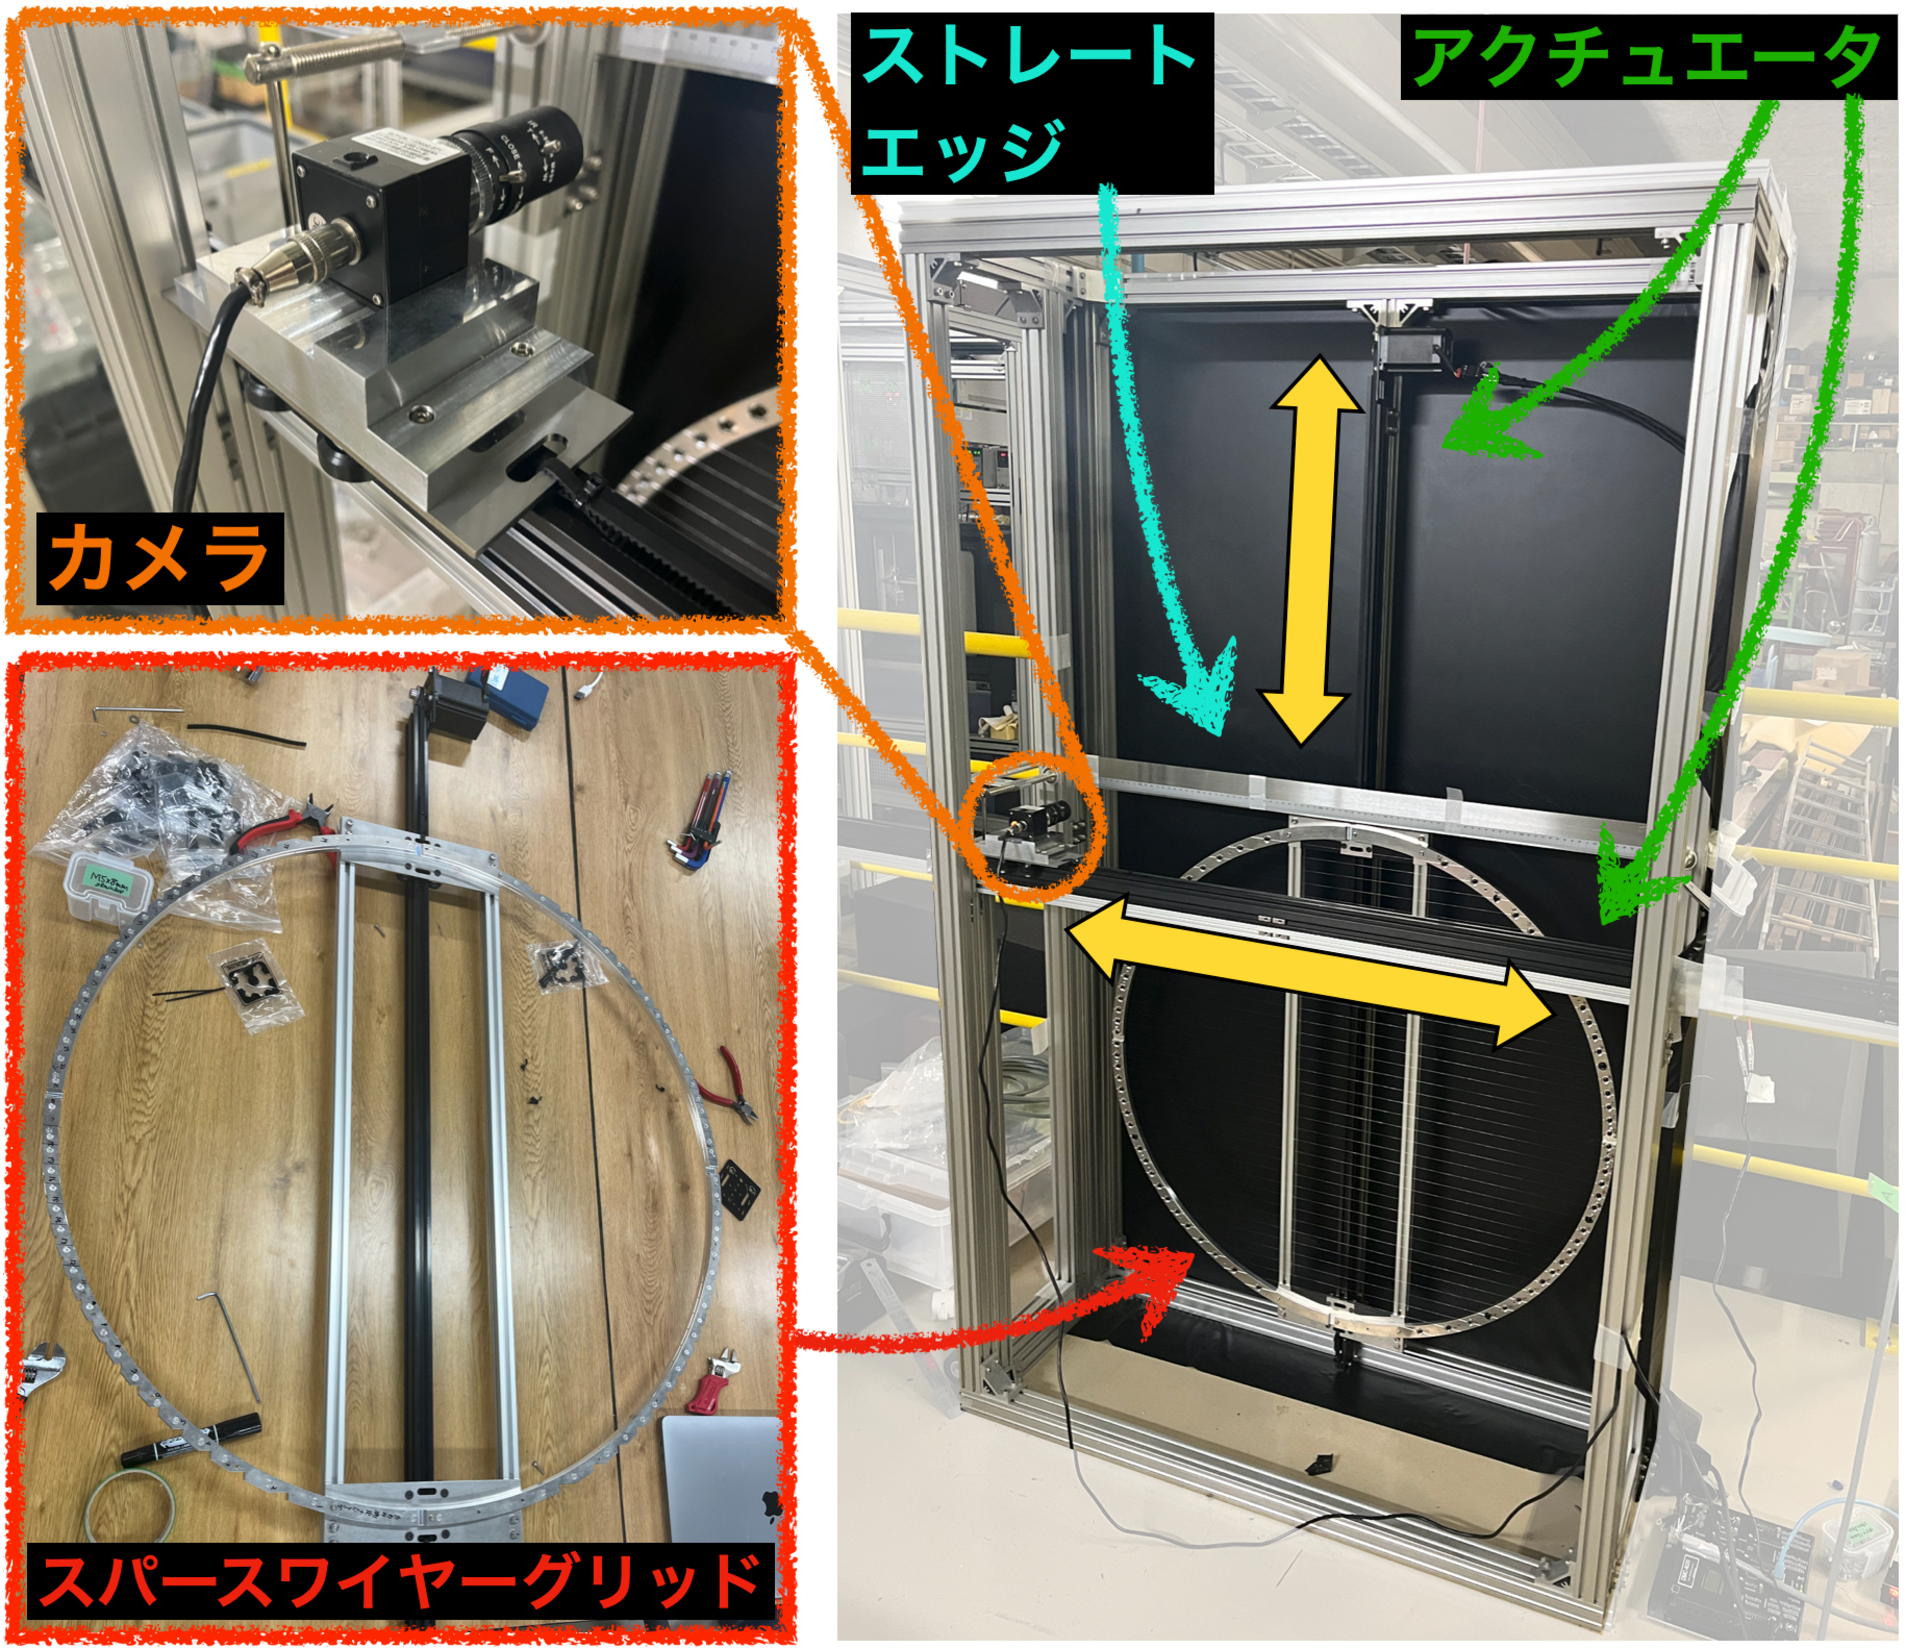
\includegraphics[width=0.8\textwidth]{wiresag/wiresag_system.pdf}
    \caption{ワイヤーのたわみ量評価系の概観}
    \label{fig:wiresag_system}
\end{figure}

\begin{figure}[H]
    \centering
    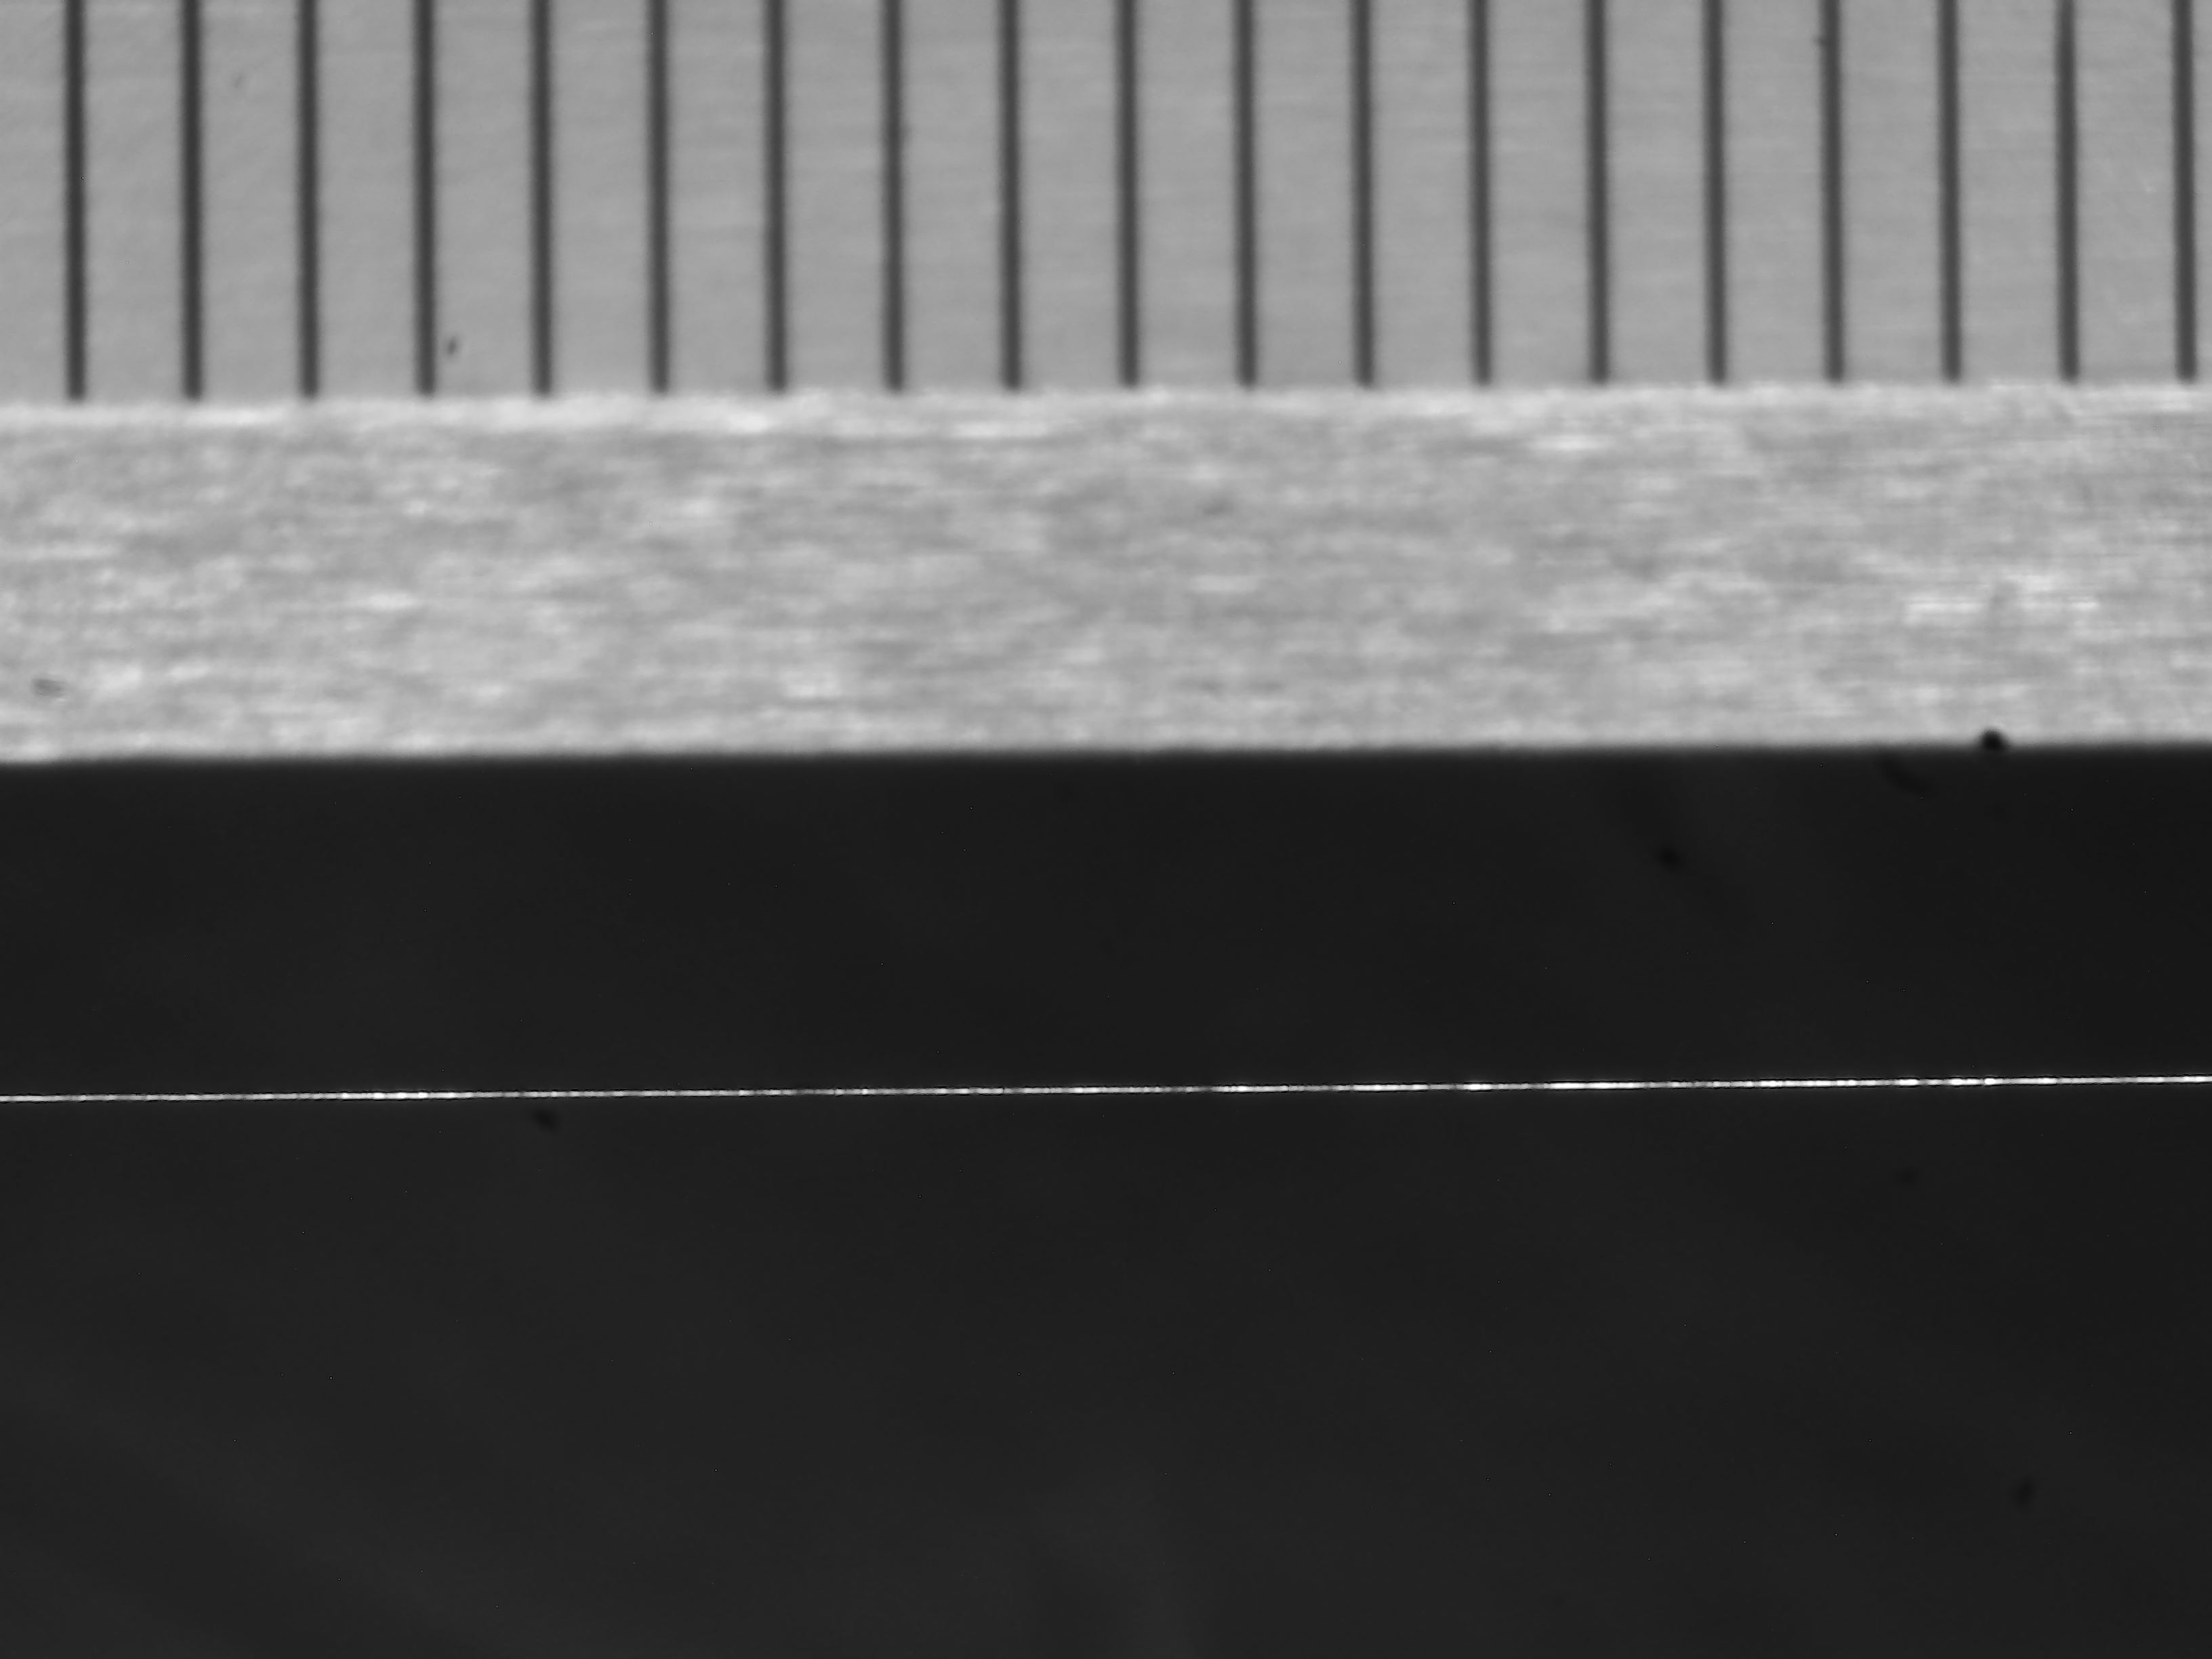
\includegraphics[width=0.7\textwidth]{wiresag/20241219_UHF_0_wire23_x467_gray.png}
    \caption{撮影されたストレートエッジとワイヤーの写真の例}
    \label{fig:wiresag_picture}    
\end{figure}

\subsection{評価原理}
\label{subsec:wiresag_principle}
まず、理想的な評価系について考える。
図\ref{fig:wiresag_concept}に評価原理の概念図を示す。
$x_{0},\,x_{1},\,\cdots,\,x_{n}$ は撮影箇所の位置を表し、$z_{0},\,z_{1},\,\cdots,\,z_{n}$ は各写真から測定されるストレートエッジとワイヤーの距離である。
得られた $x_{i},\,z_{i}$ を横軸 $x$、縦軸 $z$ でプロットすると、ワイヤーの概形を表す曲線が得られる。
ワイヤーの理論曲線はワイヤーの素材、かかっている張力により決まるカテナリー曲線であるため、
得られた曲線をカテナリー曲線で fitting することでワイヤーのたわみ量を評価することができる。

ワイヤーの概形を表すカテナリー曲線は、$T$ をワイヤーにかかる張力、$\rho_{\mathrm{W}}$ をワイヤーの密度、
$R_{\mathrm{W}}$ をワイヤーの半径、$L_{\mathrm{frame}}$ をワイヤーを固定している両端間の距離として
\begin{align}
    \label{eq:wiresag_catenary_nominal}
    f(x;a) &= a\cosh\qty(\dfrac{x+L_{\mathrm{frame}}/2}{a}) - a\cosh\qty(\dfrac{L_{\mathrm{frame}}}{2a}) \\
    a &= \dfrac{T}{\rho_{\mathrm{W}}\cdot\pi R_{\mathrm{W}}^2}
\end{align}
と表される。なお、この式は原点 $(0,\,0)$ と $(L_{\mathrm{frame}},\,0)$ を通る拘束条件を課したカテナリー曲線を表している。
スパースワイヤーグリッドにはタングステン製のワイヤーを使うため、その密度はタングステンの密度 $\rho_{\mathrm{W}}=\SI{19.3}{g/cm^3}$ であり、
ワイヤーの半径は $R_{\mathrm{W}}=\SI{0.1}{mm}$ である。
$L_{\mathrm{frame}}$ はどのワイヤーを評価するかによって異なる。
図\ref{fig:wire_number}のようにスパースワイヤーグリッドに張られたワイヤーに通し番号をつけたとき、
スパースワイヤーグリッドの内径が $\SI{790}{mm}$ であり、ワイヤー間のピッチが $\SI{20}{mm}$ であることから、
$n$ 番目のワイヤーにおける $L_{\mathrm{frame},\,n}$ は
\begin{align}
    \label{eq:wiresag_frame_length}
    L_{\mathrm{frame}, n} = 2\sqrt{395^2-(20\cdot(19-n))^2}\ [\mathrm{mm}] \quad (n=1,2,\cdots,19)
\end{align}
と表される。以下ではワイヤー番号を省略し、単純に $L_{\mathrm{frame}}$ と表す。
$a$ は張力に関わるパラメータであり、ワイヤーが緩んでいることを示す指標となる。
そのため、得られた測定値 ($x_{i},\,z_{i}$) に対して、カテナリー曲線のパラメータ $a$ を fitting parameter として
fitting を行い、best fit により得られた $a$ を用いてワイヤーのたわみ量を算出する。
式\eqref{eq:wiresag_catenary_nominal}より、張られたワイヤーの中心部で生じるたわみ量は
\begin{align}
    d_{\mathrm{sag}} &= f(L_{\mathrm{frame}}/2;a) \\
    \label{eq:wiresag_sag}
                     &= a\qty[1-\cosh\qty(\dfrac{L_{\mathrm{frame}}}{2a})]
\end{align}
であり、たわみ角 $\theta_{\mathrm{sag}}$ は
\begin{align}
    \label{eq:wiresag_sag_angle}
    \theta_{\mathrm{sag}} &= \arctan\qty(\dfrac{d_{\mathrm{sag}}}{2L_{\mathrm{frame}}})
\end{align}
となる。

\begin{figure}[H]
    \centering
    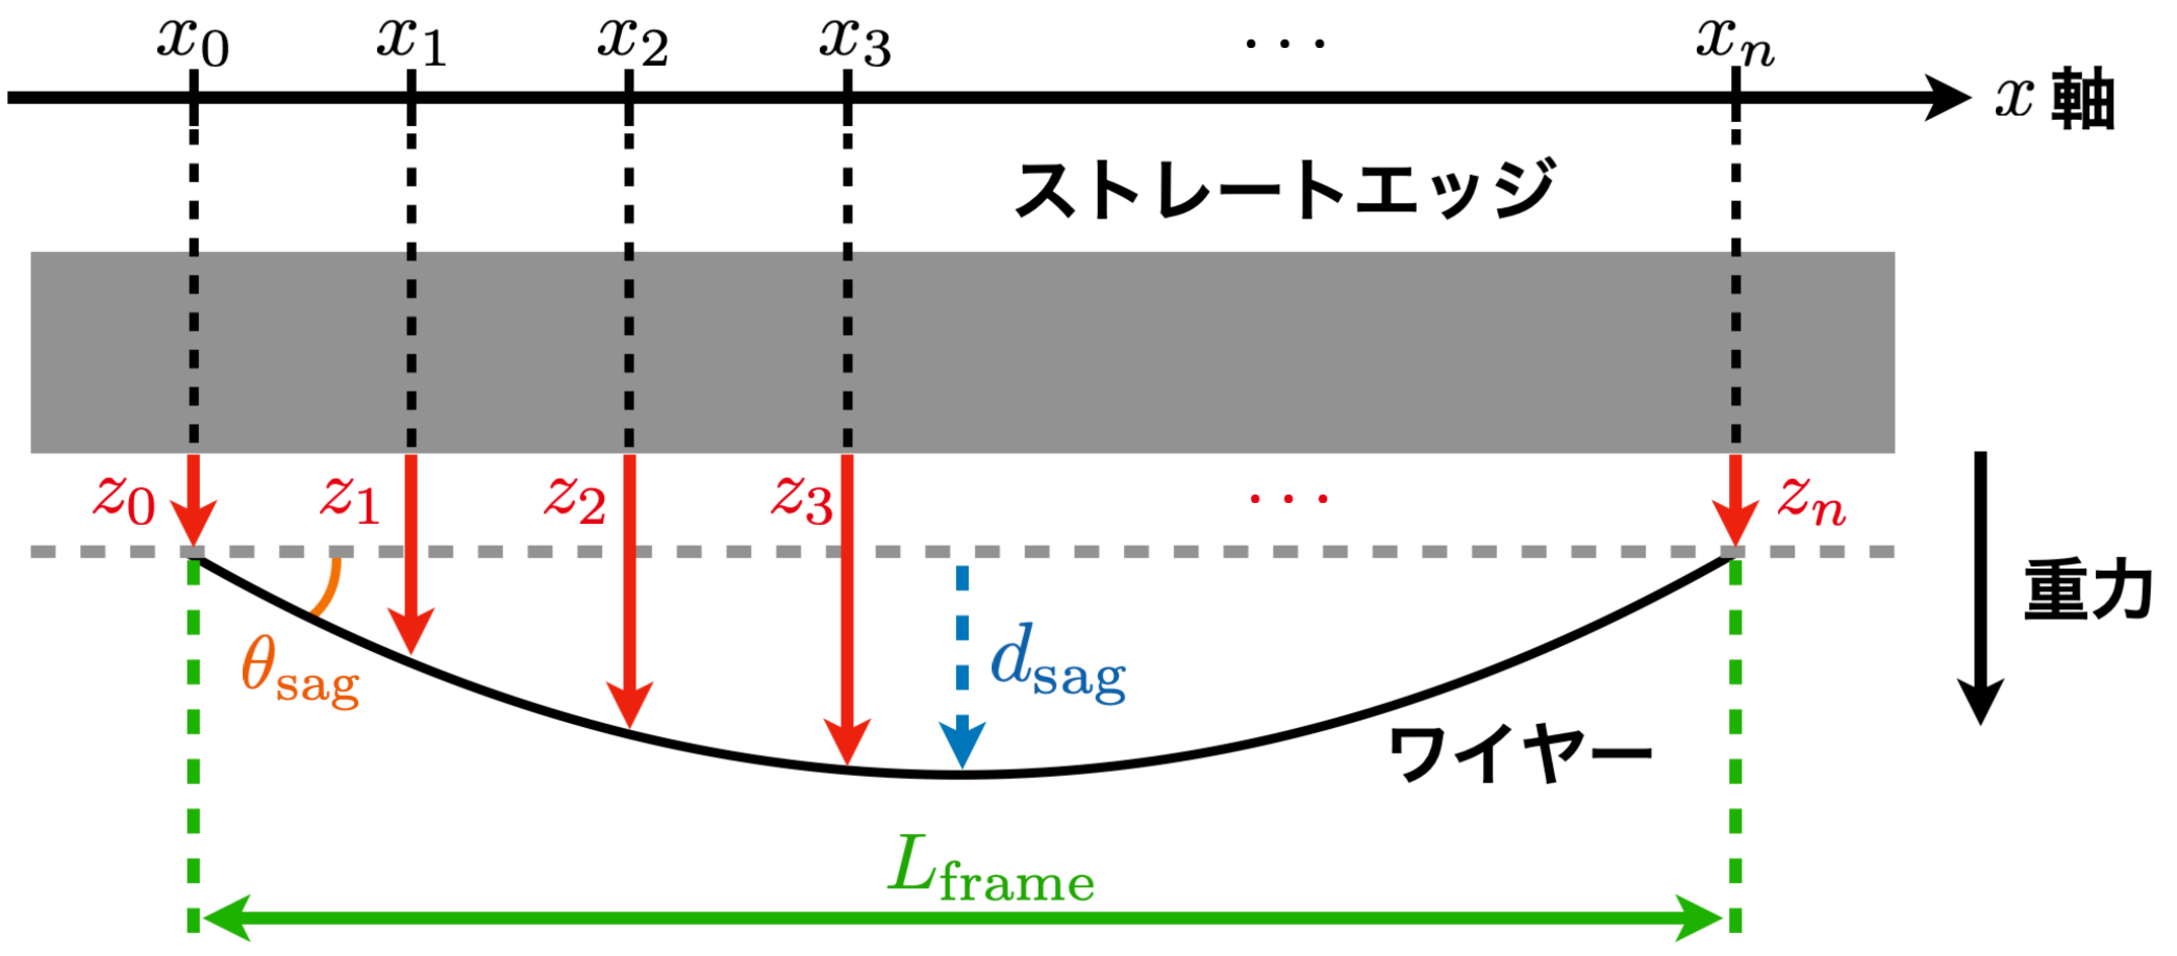
\includegraphics[width=0.8\textwidth]{wiresag/wiresag_concept.pdf}
    \caption{ワイヤーのたわみ量の評価原理}
    \label{fig:wiresag_concept}
\end{figure}
\begin{figure}[H]
    \centering
    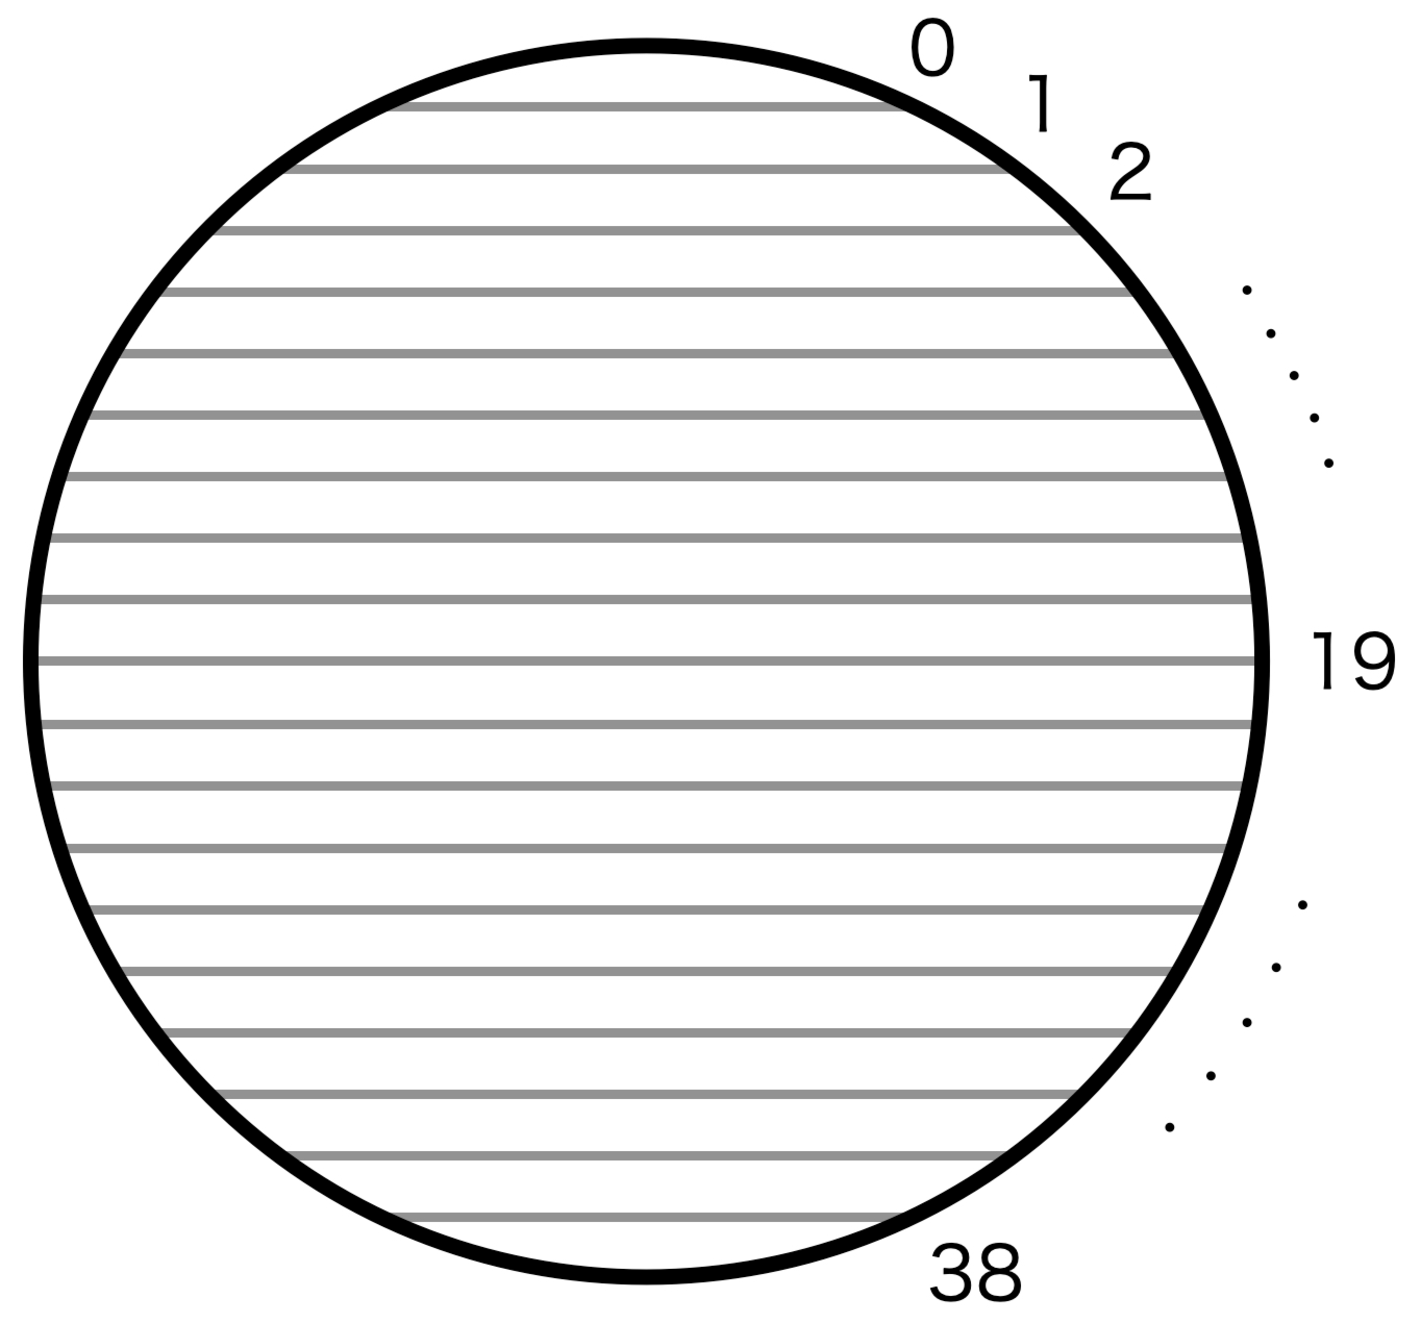
\includegraphics[width=0.5\textwidth]{wiresag/wire_number.pdf}
    \caption{スパースワイヤーグリッドにおけるワイヤー番号}
    \label{fig:wire_number}
\end{figure}

評価系が理想的でない場合について考える。
実際の評価系においてはカメラの回転、水平面からのストレートエッジの傾き、スパースワイヤーグリッドの回転により、重力方向を見誤る効果が生じる。
これは測定した $z$ が重力に沿う方向で測っていないことを意味し、その効果を消去するためには補正が必要である。
そこで、
\begin{enumerate}
    \item カメラの回転とストレートエッジの傾きによる効果
    \item スパースワイヤーグリッドの回転による効果
\end{enumerate}
と分け、それぞれの効果がどのように $z$ に影響を与えるか、もしくはどのように補正をするべきかについて考える。

\paragraph{カメラの回転とストレートエッジの傾きによる効果}\quad\\
\indent
カメラの回転による効果を消すためには、ストレートエッジが水平になるように画像を回転させればよい。
図\ref{fig:wiresag_rotation}に、回転前後のストレートエッジとワイヤーの概念図を示す。
$\theta_{\mathrm{camera}}$ はカメラの回転角を表し、 $\theta_{\mathrm{SE}}$ はストレートエッジの傾きを表す。
回転後の系においてストレートエッジに垂直な方向にワイヤーまでの距離を測り、 $z$ として算出する。
ただし、この回転はストレートエッジが傾いている効果を消去しない。
測定された $z$ と本来測るべき $z_{\mathrm{true}}$ との間にストレートエッジの傾きにより生じる誤差について考える。
図\ref{fig:wiresag_rotation}より、$z$ と $z_{\mathrm{true}}$ の関係は
\begin{align}
    z &= z_{\mathrm{true}}\cos\theta_{\mathrm{SE}} \\
    &\simeq z_{\mathrm{true}}\qty(1-\dfrac{\theta_{\mathrm{SE}}^2}{2})
\end{align}
と表される。
ストレートエッジの傾き $\theta_{\mathrm{SE}}$ は、ストレートエッジが長さ $\SI{1000}{mm}$ 
であるのに対して両端の高さのずれは多くても $\SI{10}{mm}$ 程度であることから、$\theta_{\mathrm{SE}} \sim \SI{0.01}{rad}$ と見積もられる。
したがって、$z$ と $z_{\mathrm{true}}$ の間に生じる誤差は多くとも $\SI{0.01}{\%}$ 程度であり、無視できる。

以上をまとめると、カメラの回転とストレートエッジの傾きによる効果を補正するには、ストレートエッジが水平になるように画像を回転させればよいということがわかる。
\begin{figure}[H]
    \centering
    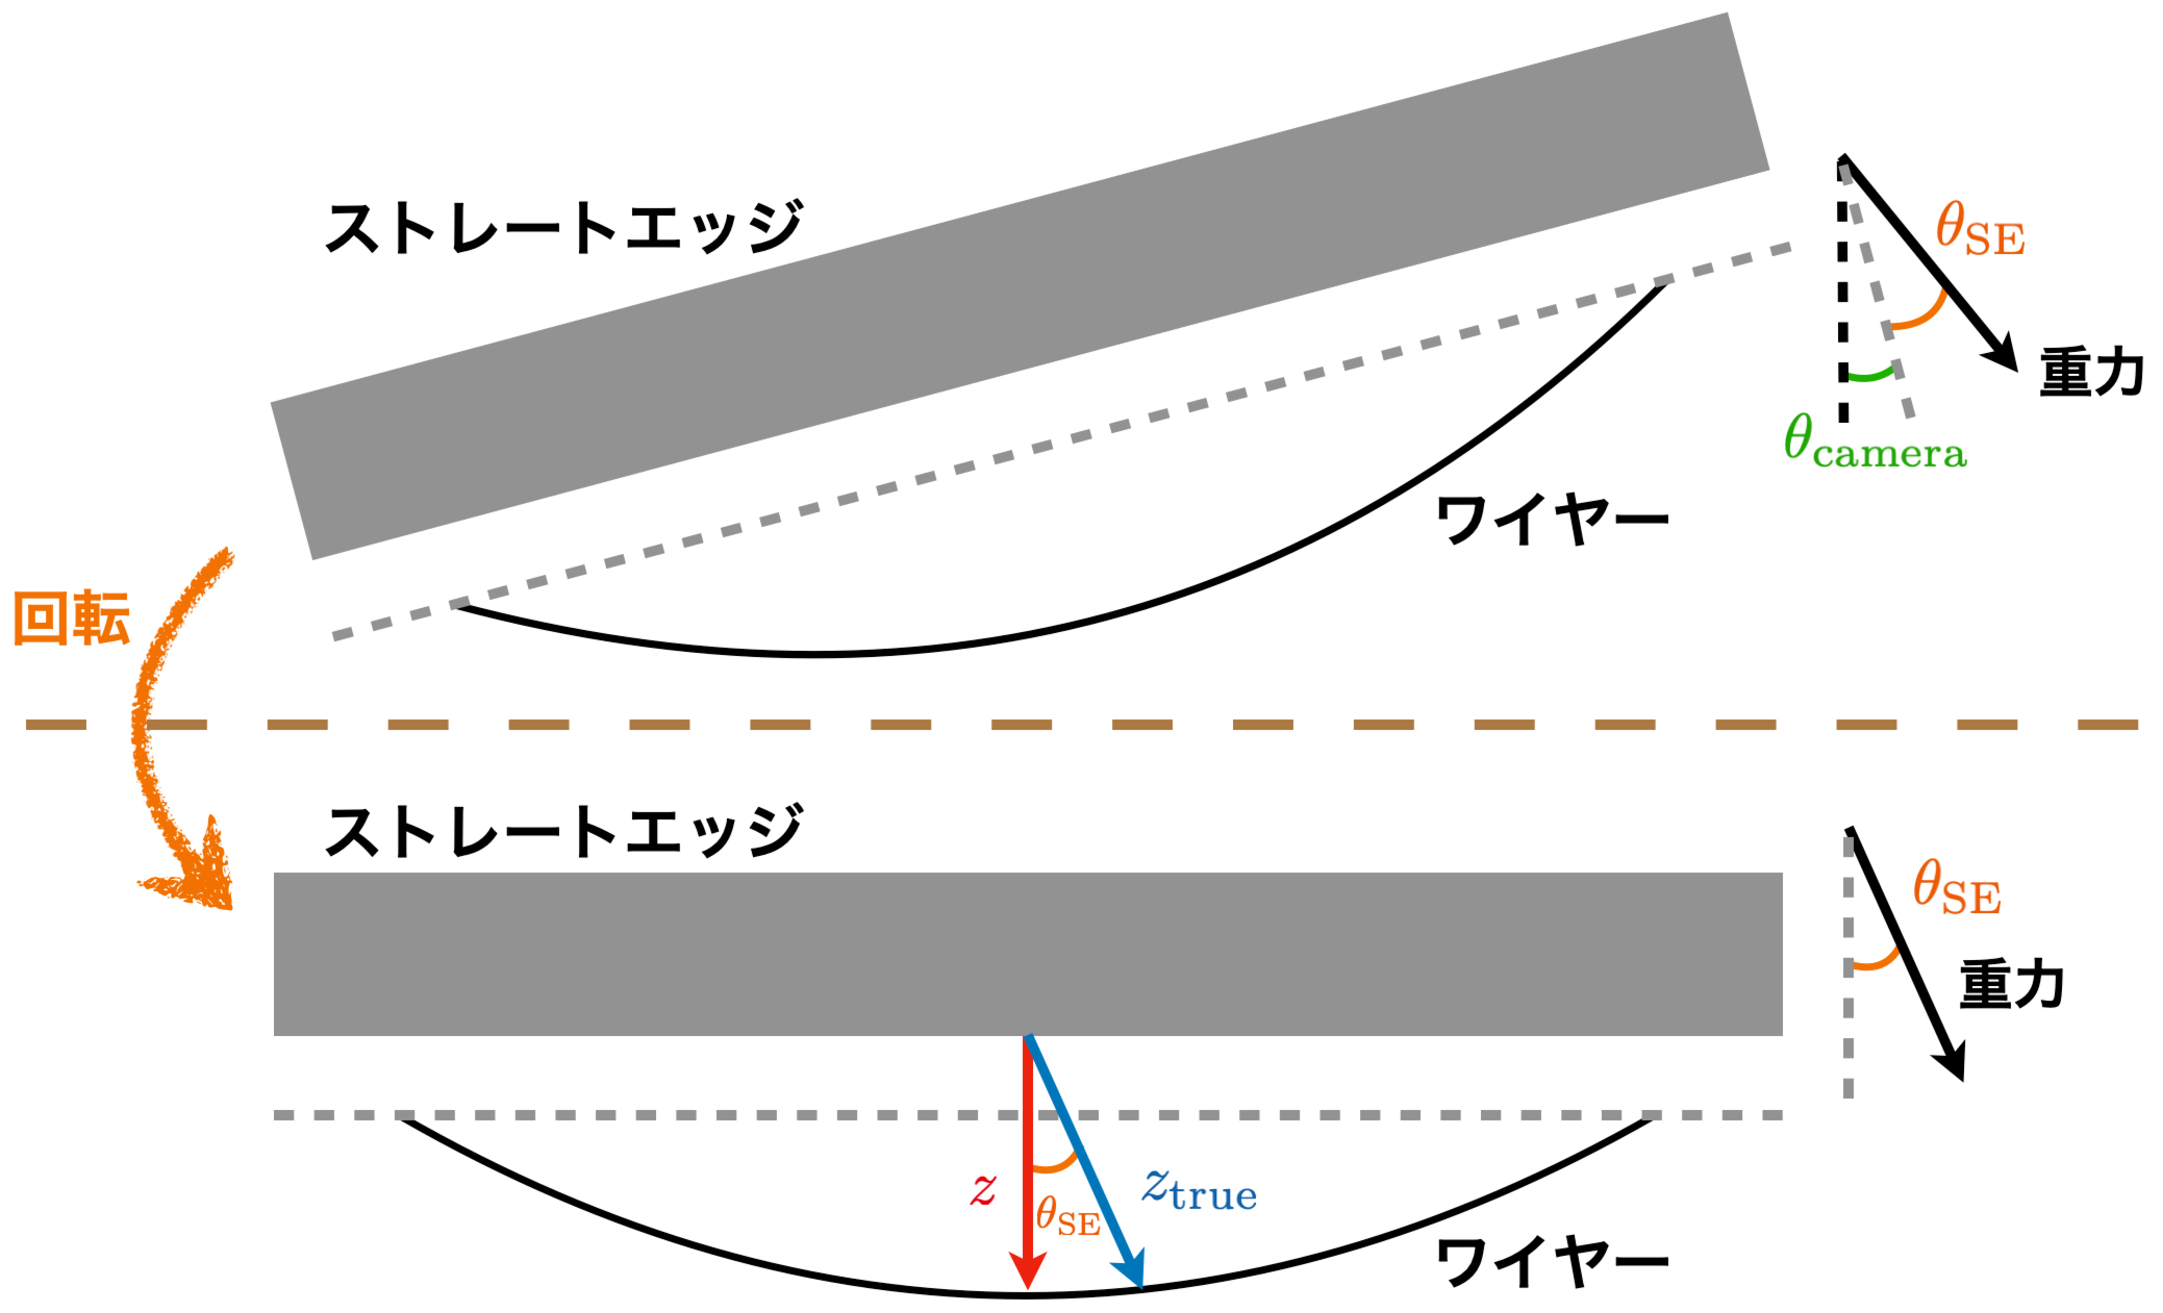
\includegraphics[width=0.8\textwidth]{wiresag/wiresag_rotation.pdf}
    \caption{ストレートエッジとワイヤーの回転前後の概念図}
    \label{fig:wiresag_rotation}
\end{figure}

\paragraph{スパースワイヤーグリッドの回転による効果}\quad\\
\indent
図\ref{fig:wiresag_concept_tilt}のように、ワイヤーの左端が $(0,\,0)$ に位置し、ワイヤーの右端が $(X,\,Y)$ に位置する場合を考える。
ワイヤーの両端を結んだ直線と $x$ 軸のなす角度が $\theta_{\mathrm{SWG}}$ であり、これはスパースワイヤーグリッドが回転している角度である。
このとき、ワイヤーの描くカテナリー曲線は
\begin{align}
    \label{eq:wiresag_catenary_tilt}
    f_{\mathrm{tilt}}(x;a,\,X,\,Y) &= a\cosh\qty(\dfrac{x+c_1}{a}) + c_2 \\
    c_1 &= a\sinh^{-1}\qty[\dfrac{Y}{2a\sinh\qty(\dfrac{X}{2a})}] \\
    c_2 &= -a\cosh\qty(\dfrac{c_1}{a})
\end{align}
となる。ただし、$X,\,Y$は
\begin{align}
    L_{\mathrm{frame}} &= \sqrt{X^2+Y^2}
\end{align}
を満たす。
測定される $z$ はストレートエッジとワイヤー間の距離であるため、その概形はカテナリー曲線を $-1$ 倍したものであり
\begin{align}
    z_{i} &= -f_{\mathrm{tilt}}(x_{i};\,a,\,X,\,Y)
\end{align}
として測定値 $(x_{i},\,z_{i})$ に対して fitting を行う。
こうして得られた $a$ を式\eqref{eq:wiresag_sag}に代入することで、ワイヤーのたわみ量 $d_{\mathrm{sag}}$ を得る。
\begin{figure}[H]
    \centering
    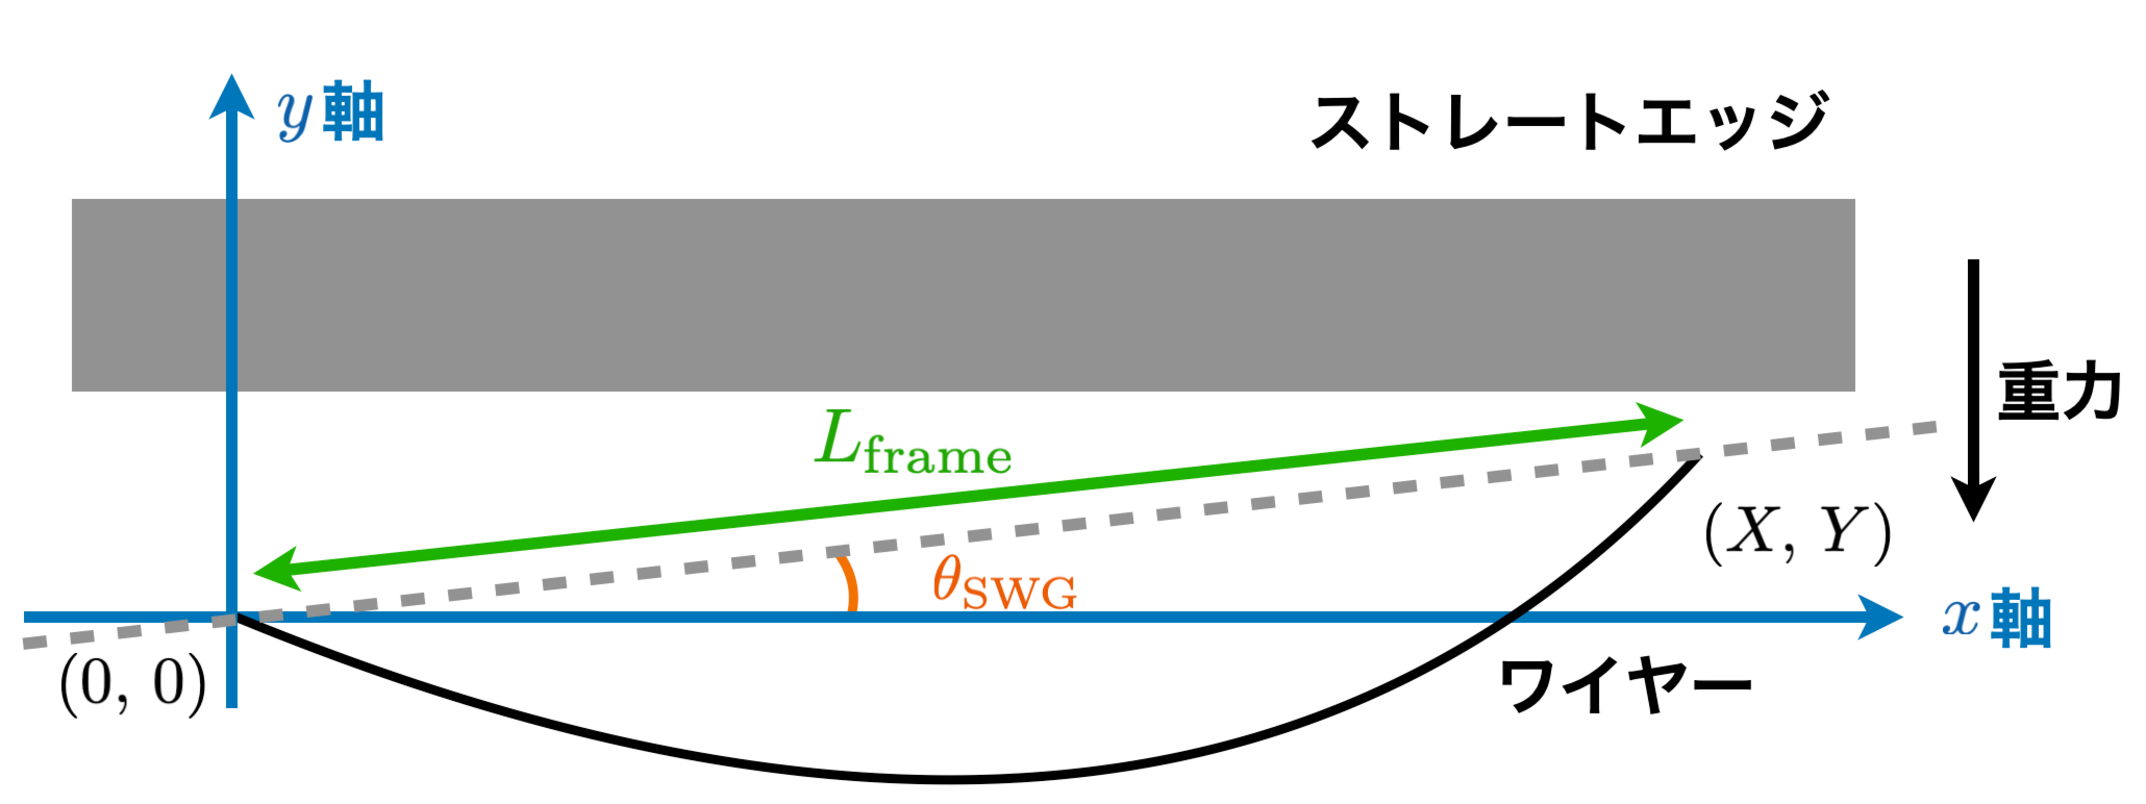
\includegraphics[width=0.8\textwidth]{wiresag/wire_catenary_tilt.pdf}
    \caption{ワイヤーの両端が重力に対して傾いている場合のワイヤーの描くカテナリーの概念図}
    \label{fig:wiresag_concept_tilt}
\end{figure}

% \subsection{評価系の光学系を考慮した $z$ の測定原理}
% 図\ref{fig:wiresag_concept_yoko}にワイヤーのたわみ量の評価原理の横から見た概念図を示す。
% これは過去の手法における概念図\ref{fig:wiresag_setup_old}を新しい系に合わせて変更したものであり、
% カメラから見るとストレートエッジが手前に位置し、ワイヤーがその奥に位置するような配置になっている。
% 各パラメータの意味とその値、誤差を表\ref{tab:wiresag_concept_yoko_params}に示す。
% この系において、測定される量 $z'$ を用いてストレートエッジとワイヤー間の距離 $z$ を表すと、
% \begin{align}
%     z = \dfrac{z'}{\cos\phi} + \alpha\tan\phi \\
%     \phi = \arctan\qty(\dfrac{L_{\mathrm{camera}}}{\alpha})
% \end{align}
% となるが、今、$L_{\mathrm{camera}}$は$\SI{0}{mm}$であるため、
% \begin{align}
%     z = z'
% \end{align}
% として問題ない。

% \begin{figure}[H]
%     \centering
%     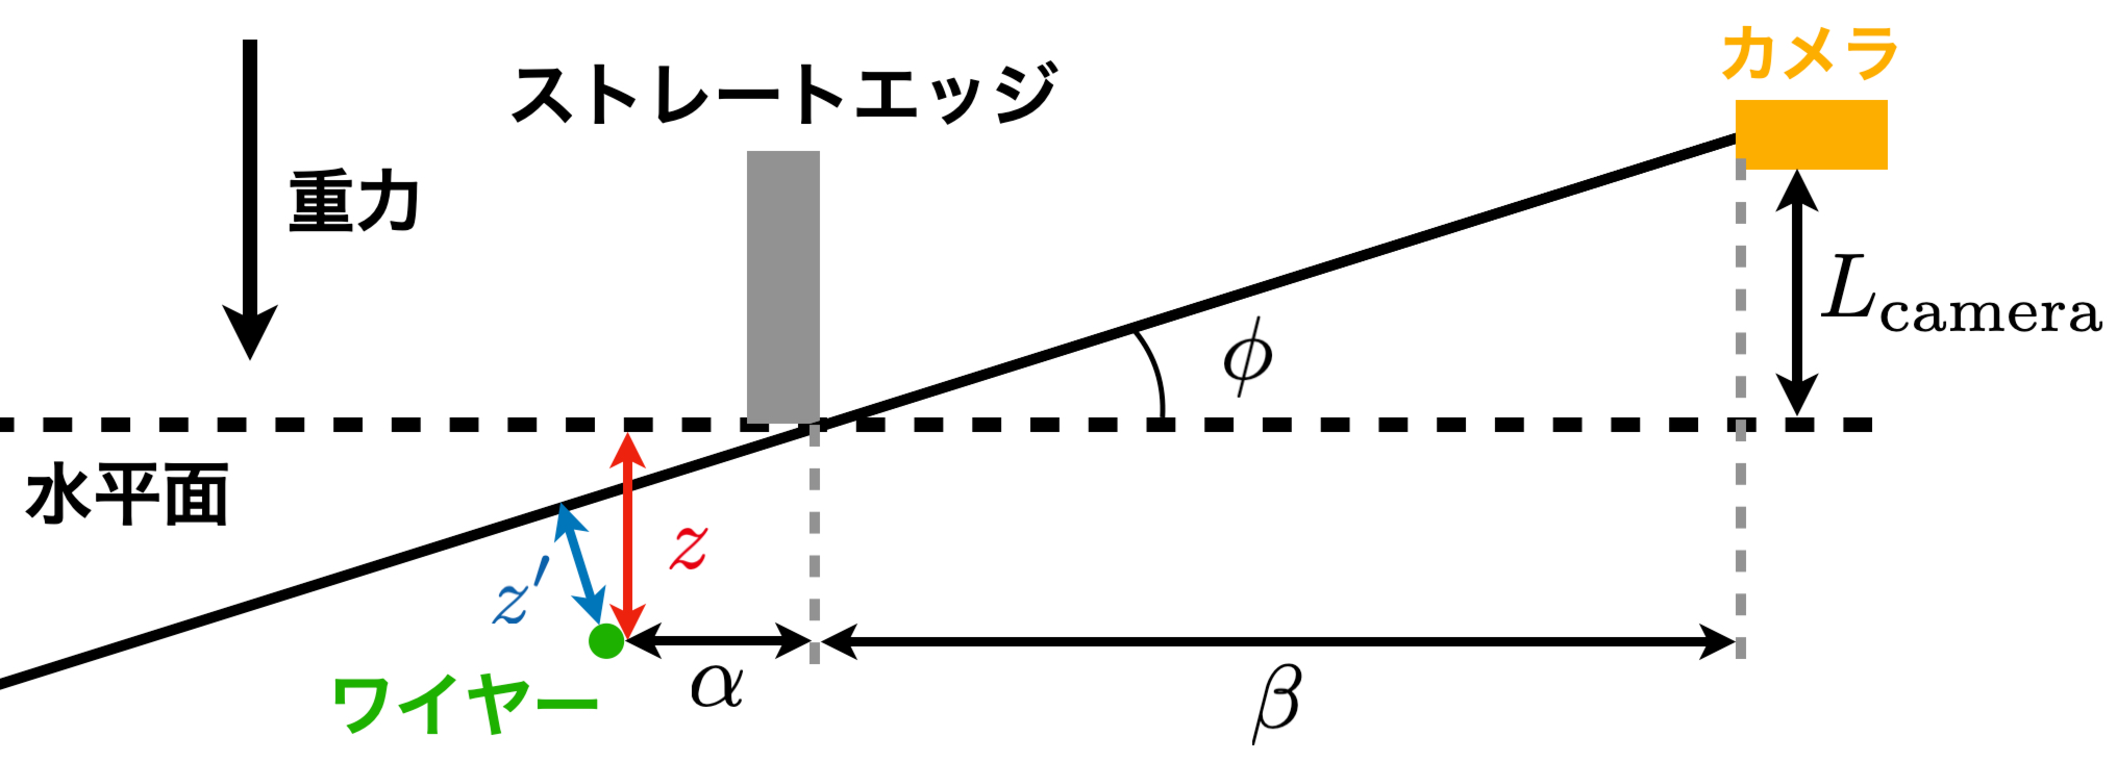
\includegraphics[width=0.8\textwidth]{wiresag/wiresag_concept_yoko.pdf}
%     \caption{ワイヤーのたわみ量の評価原理の横から見た概念図}
%     \label{fig:wiresag_concept_yoko}
% \end{figure}
% \begin{table}[H]
%     \centering
%     \caption{図\ref{fig:wiresag_concept_yoko}における各パラメータの意味と値}
%     \begin{tabular}{cccc}
%         \hline
%         パラメータ & 意味 & 値 & 誤差 \\
%         \hline\hline
%         $\alpha$ & ストレートエッジとワイヤーまでの水平距離 & $\SI{15}{mm}$ & $\pm\SI{2}{mm}$ \\
%         $\beta$ & ストレートエッジからカメラまでの水平距離 & $\SI{205}{\mm}$ & $\pm\SI{5}{mm}$ \\
%         $L_{\mathrm{camera}}$ & ストレートエッジ下端の面からカメラまでの鉛直距離 & $\SI{0}{mm}$ & $\pm\SI{0.5}{mm}$ \\
%         \hline
%     \end{tabular}
%     \label{tab:wiresag_concept_yoko_params}
% \end{table}

% \subsection{評価系の設計から生まれる $z$ の誤差の見積もり}
% 過去の手法においては、$\phi$ が典型的に $5\tcdegree$ 程度と小さくない値であったために、
% $L_{\mathrm{camera}}$ や $\alpha$ から $z$ へ大きな誤差が生じていた\cite{swg:murata}。
% この誤差を抑えるためには、$\phi$ を小さくすることが重要であるが、
% 過去の評価系ではスパースワイヤーグリッドを水平面上に設置して撮影しており、
% 他のワイヤーが撮影対象のワイヤーに重なってしまうため $\phi\sim 0\tcdegree$、すなわち 
% $L_{\mathrm{camera}} \sim \SI{0}{mm}$ で撮影することができなかった(図\ref{fig:wiresag_picture_old})。
% これを解決するため、スパースワイヤーグリッドを鉛直方向に立てて撮影を行うことで、$L_{\mathrm{camera}}=0\pm\SI{0.5}{mm}$ で撮影を行い、誤差の低減を図った。
% 新しい評価系において、$z$ の誤差は
% \begin{align}
%     \delta z = \sqrt{\qty(\dfrac{1}{\cos\phi})^2\delta z'^2 + \qty(\dfrac{\tan\phi}{\cos\phi}+\dfrac{\alpha}{\cos^2\phi})^2\delta\phi^2 + \tan^2\phi\delta\alpha^2}
% \end{align}
% と表され、表\ref{tab:wiresag_concept_yoko_params}に示したパラメータの誤差を代入すると、
% \begin{equation}
%     \delta z \sim \SI{39}{\mu m}
% \end{equation}
% となる。$z'$ の誤差についてはカメラの $\SI{1}{pixel}$ が対応する長さであり、
% 次節の解析にて明らかになるがこれは典型的に $5\sim\SI{6}{\mu m}$ 程度である。
% また、$z$ にはストレートエッジの真直度由来の誤差 $\SI{30}{\mu m}$ が含まれるため、これも考慮に入れると $z$ の誤差は
% \begin{equation}
%     \delta z = \sqrt{39^2+30^2}\ \mu\mathrm{m} = \SI{49}{\mu m}
% \end{equation}
% 程度だと見積もられる。

\section{解析手法}
\subsection{解析の流れ}
撮影された画像は既に図\ref{fig:wiresag_picture}にて示した。この図を例として、実際に行う解析の流れを説明する。
画像の解像度は $\SI{3264}{pixel}\times\SI{2448}{pixel}$ である。
画像の横軸を $x_{\mathrm{pix}}$、縦軸を $y_{\mathrm{pix}}$ と定め、画像の左上を原点 $(0,\,0)$ とする。
また、画像の出力フォーマットは yuyv であり、これは各pixelの輝度に関する情報を失うことなく保存される。
一枚の画像に対して代表的なストレートエッジとワイヤー間の距離 $z$ を算出し、たわみ量を評価するため、輝度の情報を用いて以下の手順で解析を行う。
\begin{enumerate}
    \item スケーラの目盛の輝度をfittingし、その間隔のpixel数を求めることで画像の 1 pixel が対応する長さを決める
    \item ストレートエッジの下端の輝度をfittingし、その位置を決める
    \item ストレートエッジの下端が水平になるように画像を回転させる
    \item ワイヤーの輝度をfittingし、ワイヤーの位置を決める
    \item 回転したストレートエッジの位置とワイヤーの位置から $z$ を算出する
    \item 複数の写真から得られた $z$ をカテナリー曲線で fitting し、ワイヤーのたわみ量を算出する
\end{enumerate}

\subsection{スケーラのfitting}
図\ref{fig:wiresag_scaler_target}、図\ref{fig:wiresag_scaler_brightness}に
$y_{\mathrm{pix}}=\SI{200}{pixel}$ における輝度を示す。
図\ref{fig:wiresag_scaler_brightness}では、横軸を $\SI{1100}{pixel} \leq x_{\mathrm{pix}} \leq \SI{1700}{pixel}$
に拡大したものを合わせて示している。
スケーラの目盛は黒く塗られており、その間は金属により光を反射しているため、その輝度は目盛上で低く、目盛間で高くなる。
理想的には、この輝度の変化は階段関数的である。
一つの目盛とその周りに対して、その輝度は目盛上で低く $B_{\mathrm{scaler}}^{\mathrm{single}}(x)$ は
\begin{align}
    B_{\mathrm{scaler,\,ideal}}^{\mathrm{single}}(x) &= a\qty[\theta(x-x_{\mathrm{left}})+\theta(x_{\mathrm{right}}-x)] + \mathrm{offset} \\
    \theta(x) &= \begin{cases}
        1 & (x>0) \\
        0 & (x\leq 0)
    \end{cases}
\end{align}
のように表せる。$a$ は輝度の最大値と最小値の差からくるパラメータであり、$x_{\mathrm{left}},\,x_{\mathrm{right}}$ は目盛の左端と右端の位置、$\mathrm{offset}$ は輝度のオフセットである。
しかし、実際には写真のピントにより輝度がぼやけてしまい、図\ref{fig:wiresag_scaler_brightness} のように滑らかに輝度が変化する。
そこで、この階段関数をシグモイド間数に置き換えることでこの輝度の変化をモデル化する。
\begin{align}
    &B_{\mathrm{scaler}}^{\mathrm{single}}(x;\,a,\,b,\,c,\,d,\,\mathrm{offset}) = \notag \\
        &\qquad\qquad a\qty[\dfrac{1}{1+\exp\qty(-b\qty(x-c-d))} + \dfrac{1}{1+\exp\qty(-b\qty(-x-c+d))}] + \mathrm{offset}
\end{align}
$a,\,b,\,c,\,d,\,\mathrm{offset}$ は fitting parameter であり、 $d$ は目盛の中心を表す。
さらに、写真中には複数のスケーラが写っているため、最終的にスケーラの輝度のfitting関数 $B_{\mathrm{scaler}}$ は
\begin{align}
    &B_{\mathrm{scaler}}(x;\,a_i,\,b_i,\,c_i,\,d_i,\,\text{offset}) = \notag\\
    &\qquad\qquad\sum_{i=1}^{n_{\mathrm{scaler}}} a_i\qty[\dfrac{1}{1+\exp\qty(-b_i\qty(x-c_i-d_i))} + \dfrac{1}{1+\exp\qty(-b_i\qty(-x-c_i+d_i))}] + \mathrm{offset}
\end{align}
と表される。$n_{\mathrm{scaler}}$ は写真中に写っているスケーラの数であり、offsetはすべての目盛に対して共通のパラメータである。
\begin{figure}[H]
    \centering
    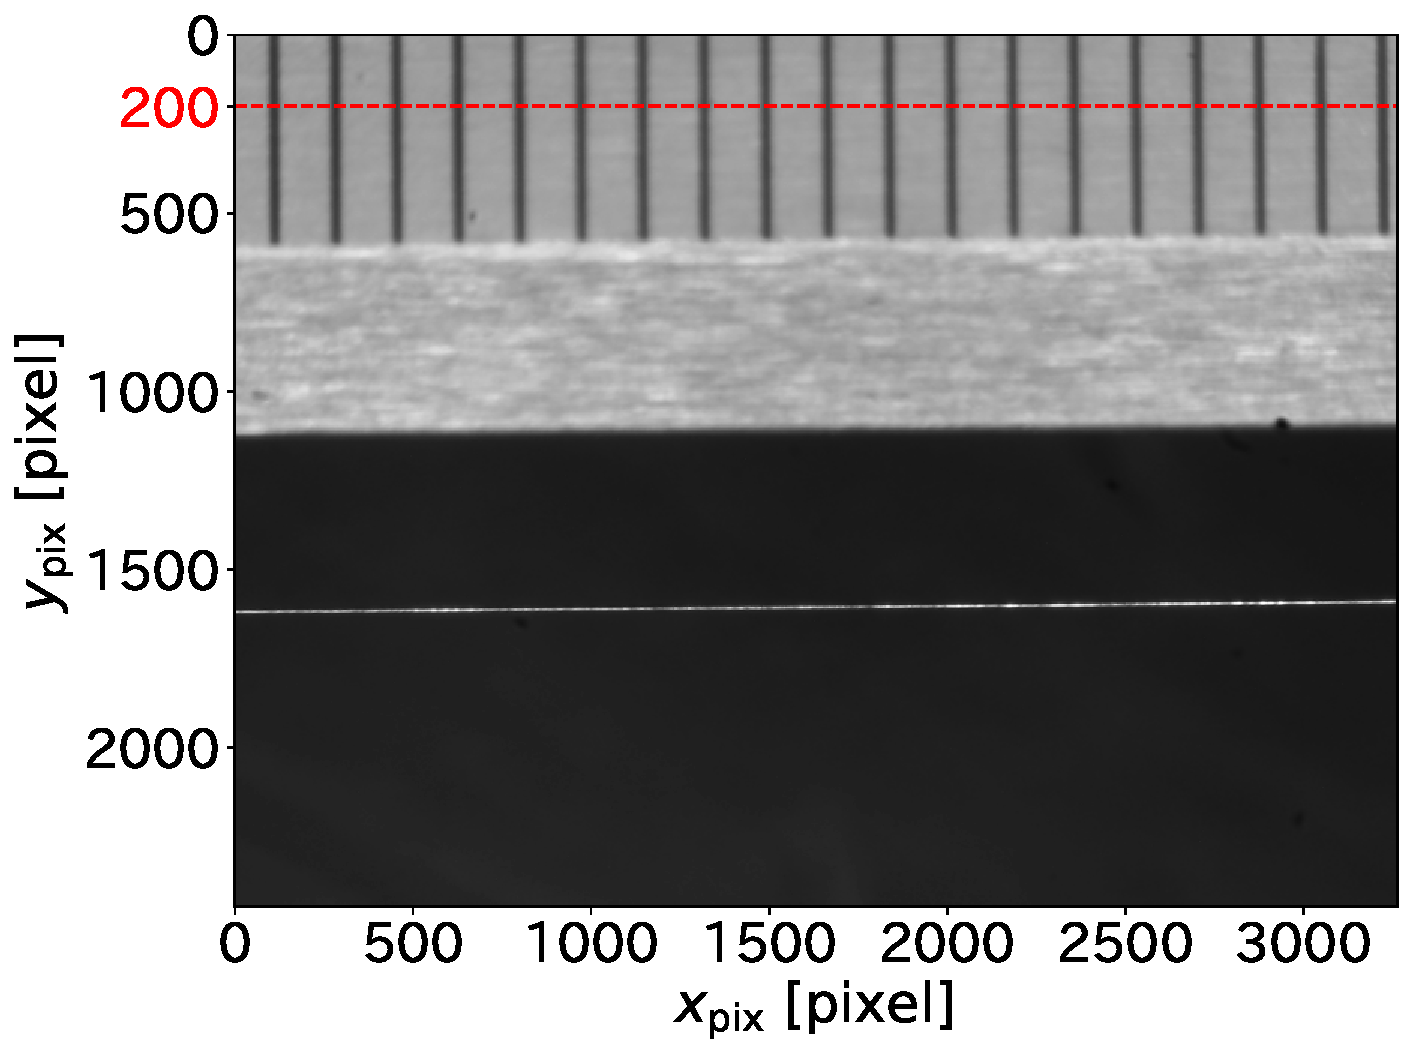
\includegraphics[width=0.8\textwidth]{wiresag/wiresag_scaler_target.pdf}
    \caption{写真中における $y_{\mathrm{pix}}=\SI{200}{pixel}$ の目安}
    \label{fig:wiresag_scaler_target}
\end{figure}
\begin{figure}[H]
    \centering
    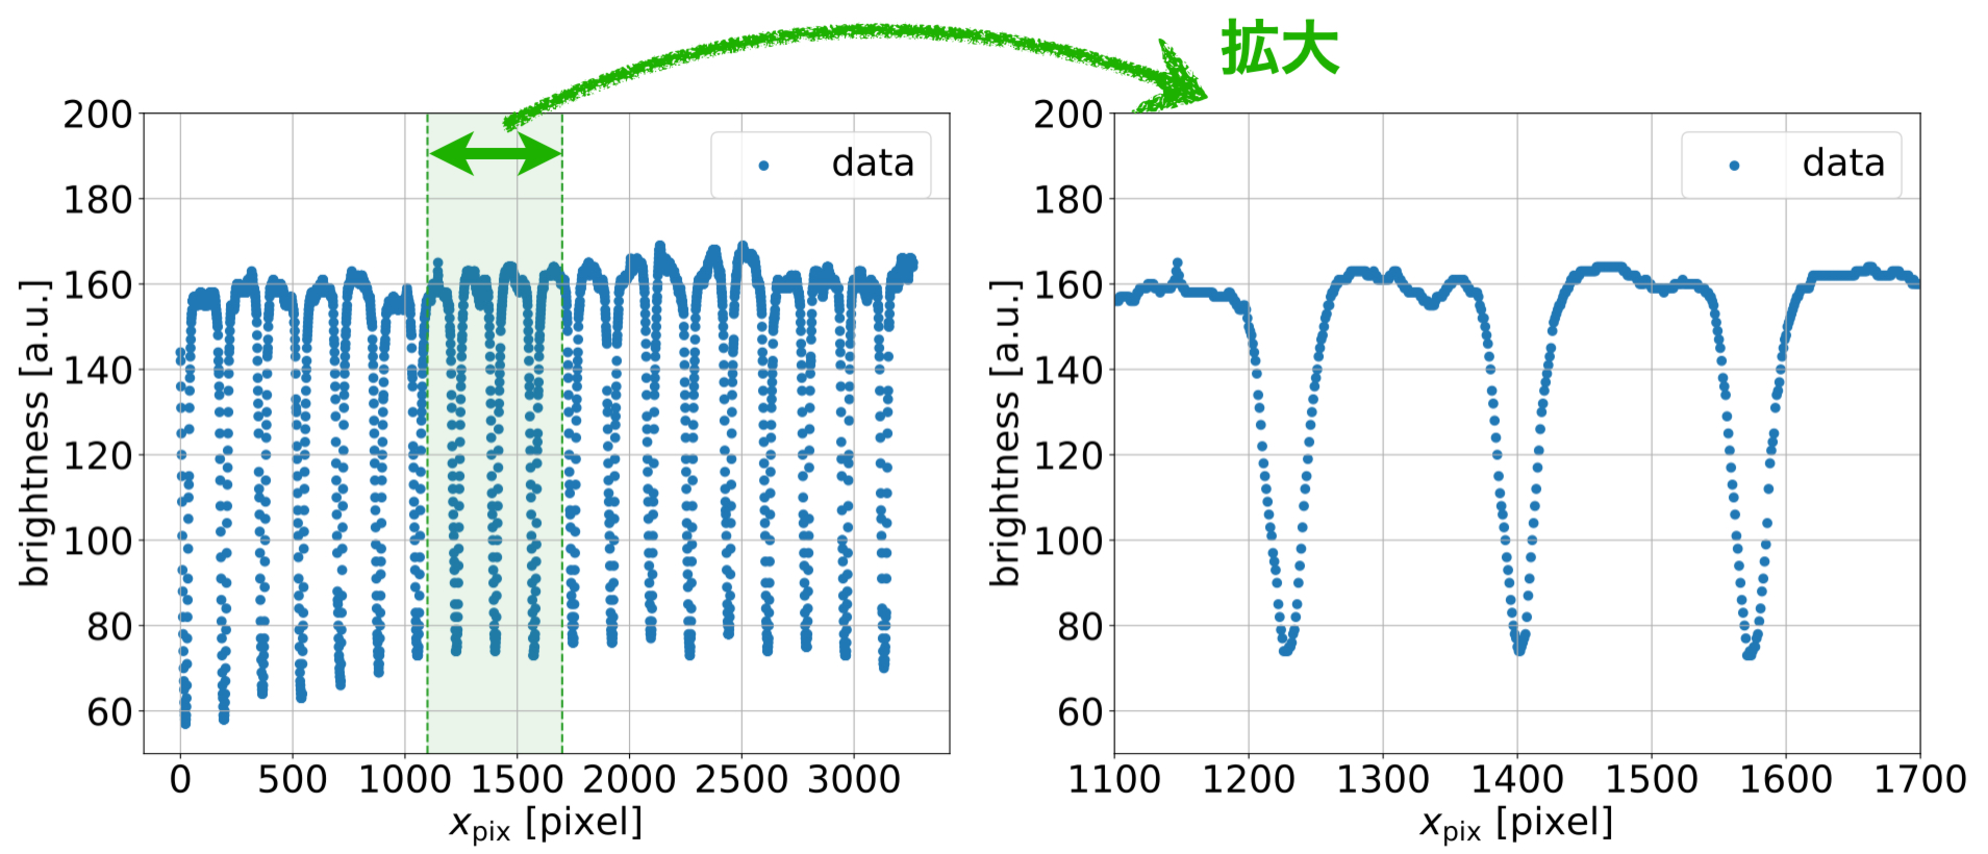
\includegraphics[width=1.0\textwidth]{wiresag/wiresag_scaler_brightness.pdf}
    \caption{$y_{\mathrm{pix}}=\SI{200}{pixel}$ における輝度の例}
    \label{fig:wiresag_scaler_brightness}
\end{figure}

図\ref{fig:wiresag_scaler_fitting}に実際にfittingした結果を示す。
$d_i$ の fitting error は典型的に $\SI{0.02}{pixel}$ 程度であった。
fittingに求められた $d_i$ から、目盛間の pixel 数を求めると、その平均は $\SI{173}{pixel}$、誤差は $\SI{0.007}{pixel}$ であった。
目盛間は $\SI{1}{mm}$ であるため、1 pixel が対応する長さは $\SI{5.78}{\mu m}\,\pm\,\SI{2e-4}{\mu m}$ となった。
\begin{figure}[H]
    \centering
    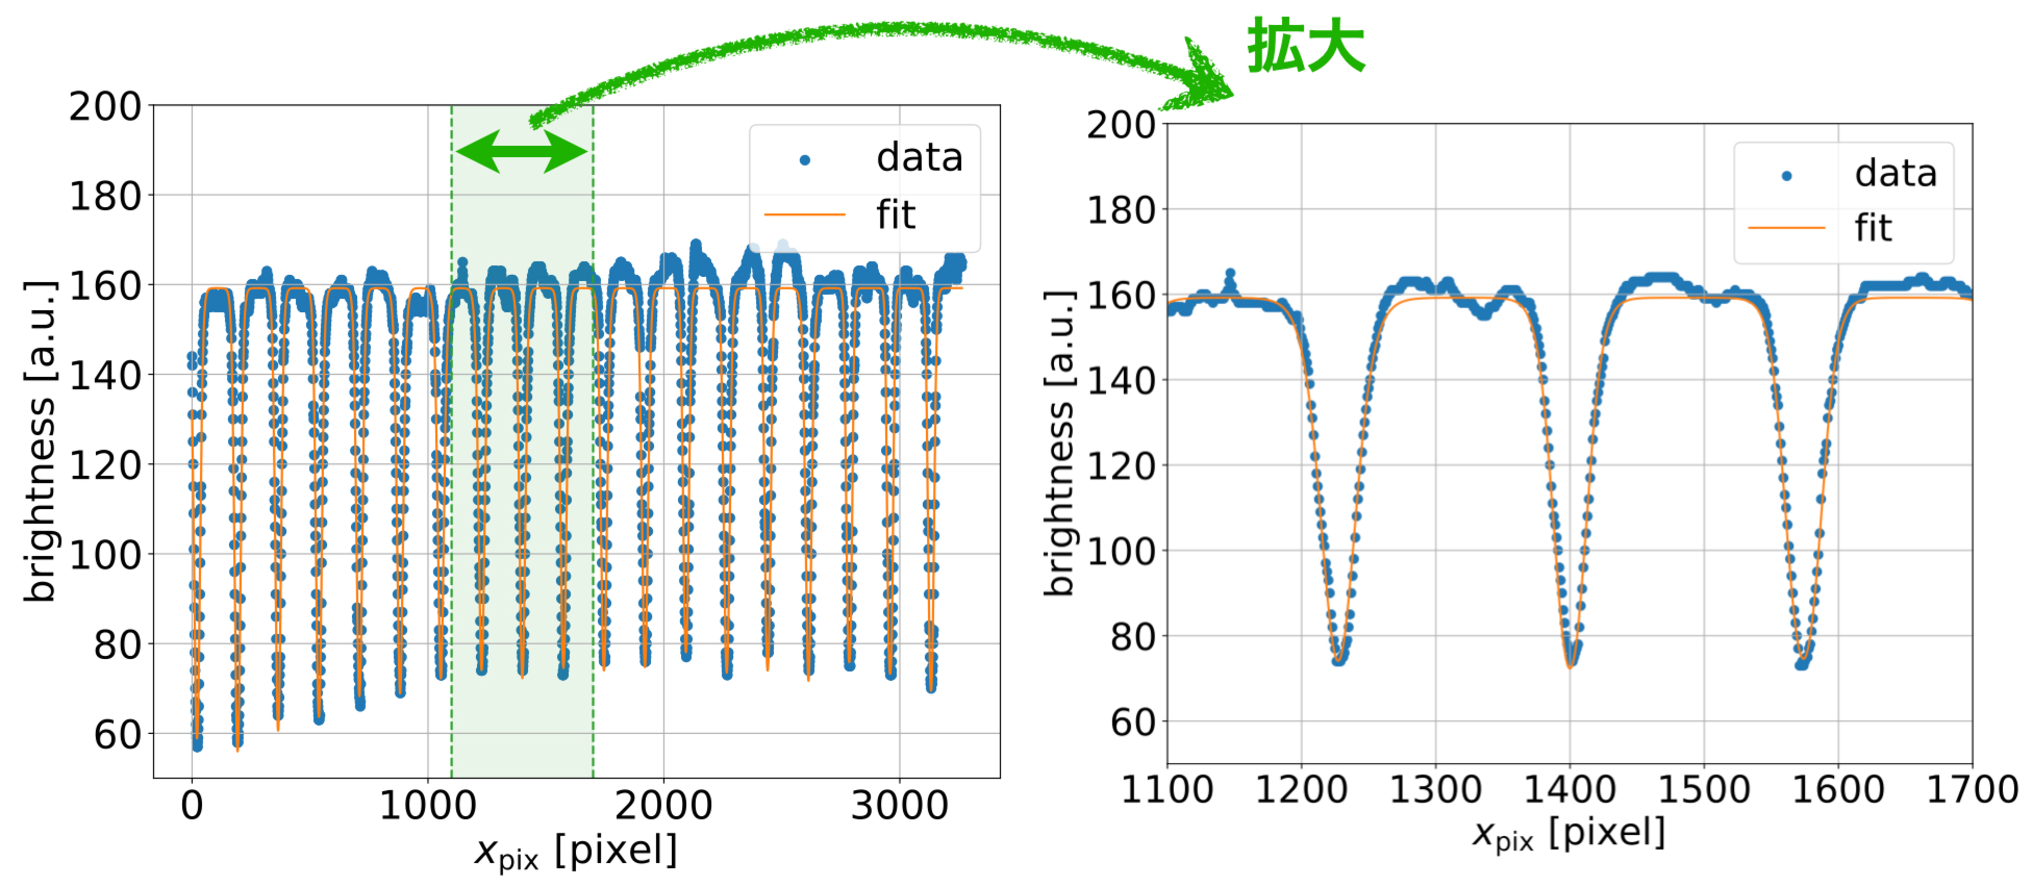
\includegraphics[width=1.0\textwidth]{wiresag/wiresag_scaler_fitting.pdf}
    \caption{$y_{\mathrm{pix}}=\SI{200}{pixel}$ スケーラの輝度のfittingの結果の例}
    \label{fig:wiresag_scaler_fitting}
\end{figure}

\subsection{ストレートエッジとワイヤーのfitting}
図\ref{fig:wiresag_edge_target}、図\ref{fig:wiresag_edge_brightness}に、$x_{\mathrm{pix}}=\SI{1665}{pixel}$ における輝度を示す。
図\ref{fig:wiresag_edge_brightness}において、$x_{\mathrm{pix}}<600$ あたりの緑でマスクされた輝度が低いところはスケーラの目盛の部分を表しており、
$600 < x_{\mathrm{pix}} < 1100$ あたりの赤でマスクされた輝度が高くなっている部分がストレートエッジの表面を、その後再び急激に低くなるところがストレートエッジの下端を表している。
また、$1550 < x_{\mathrm{pix}} < 1650$ あたりのオレンジでマスクされた輝度が急上昇、急降下している部分がワイヤーを表している。
\begin{figure}[H]
    \centering
    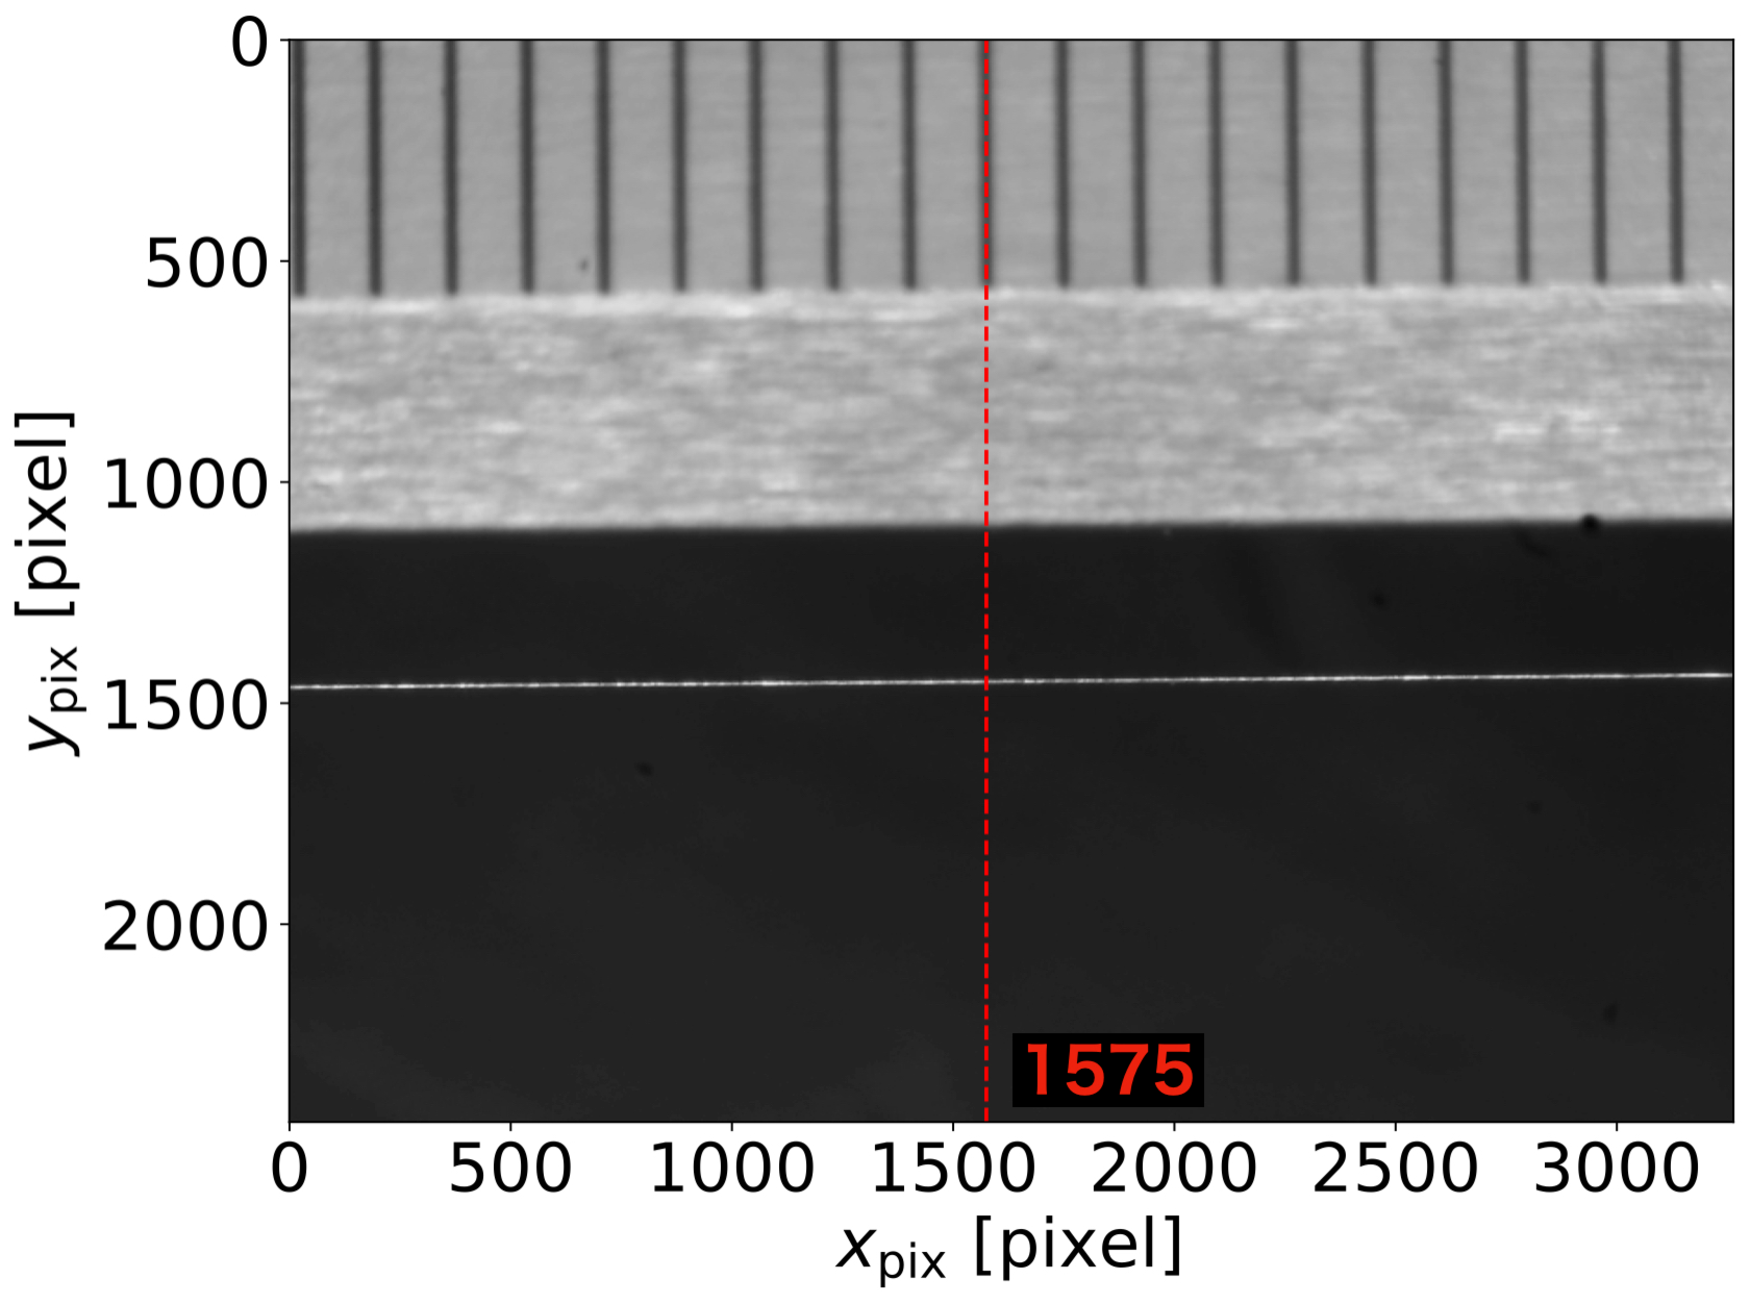
\includegraphics[width=0.8\textwidth]{wiresag/wiresag_edge_target.pdf}
    \caption{写真中における $x_{\mathrm{pix}}=\SI{1665}{pixel}$ の目安}
    \label{fig:wiresag_edge_target}
\end{figure}
\begin{figure}[H]
    \centering
    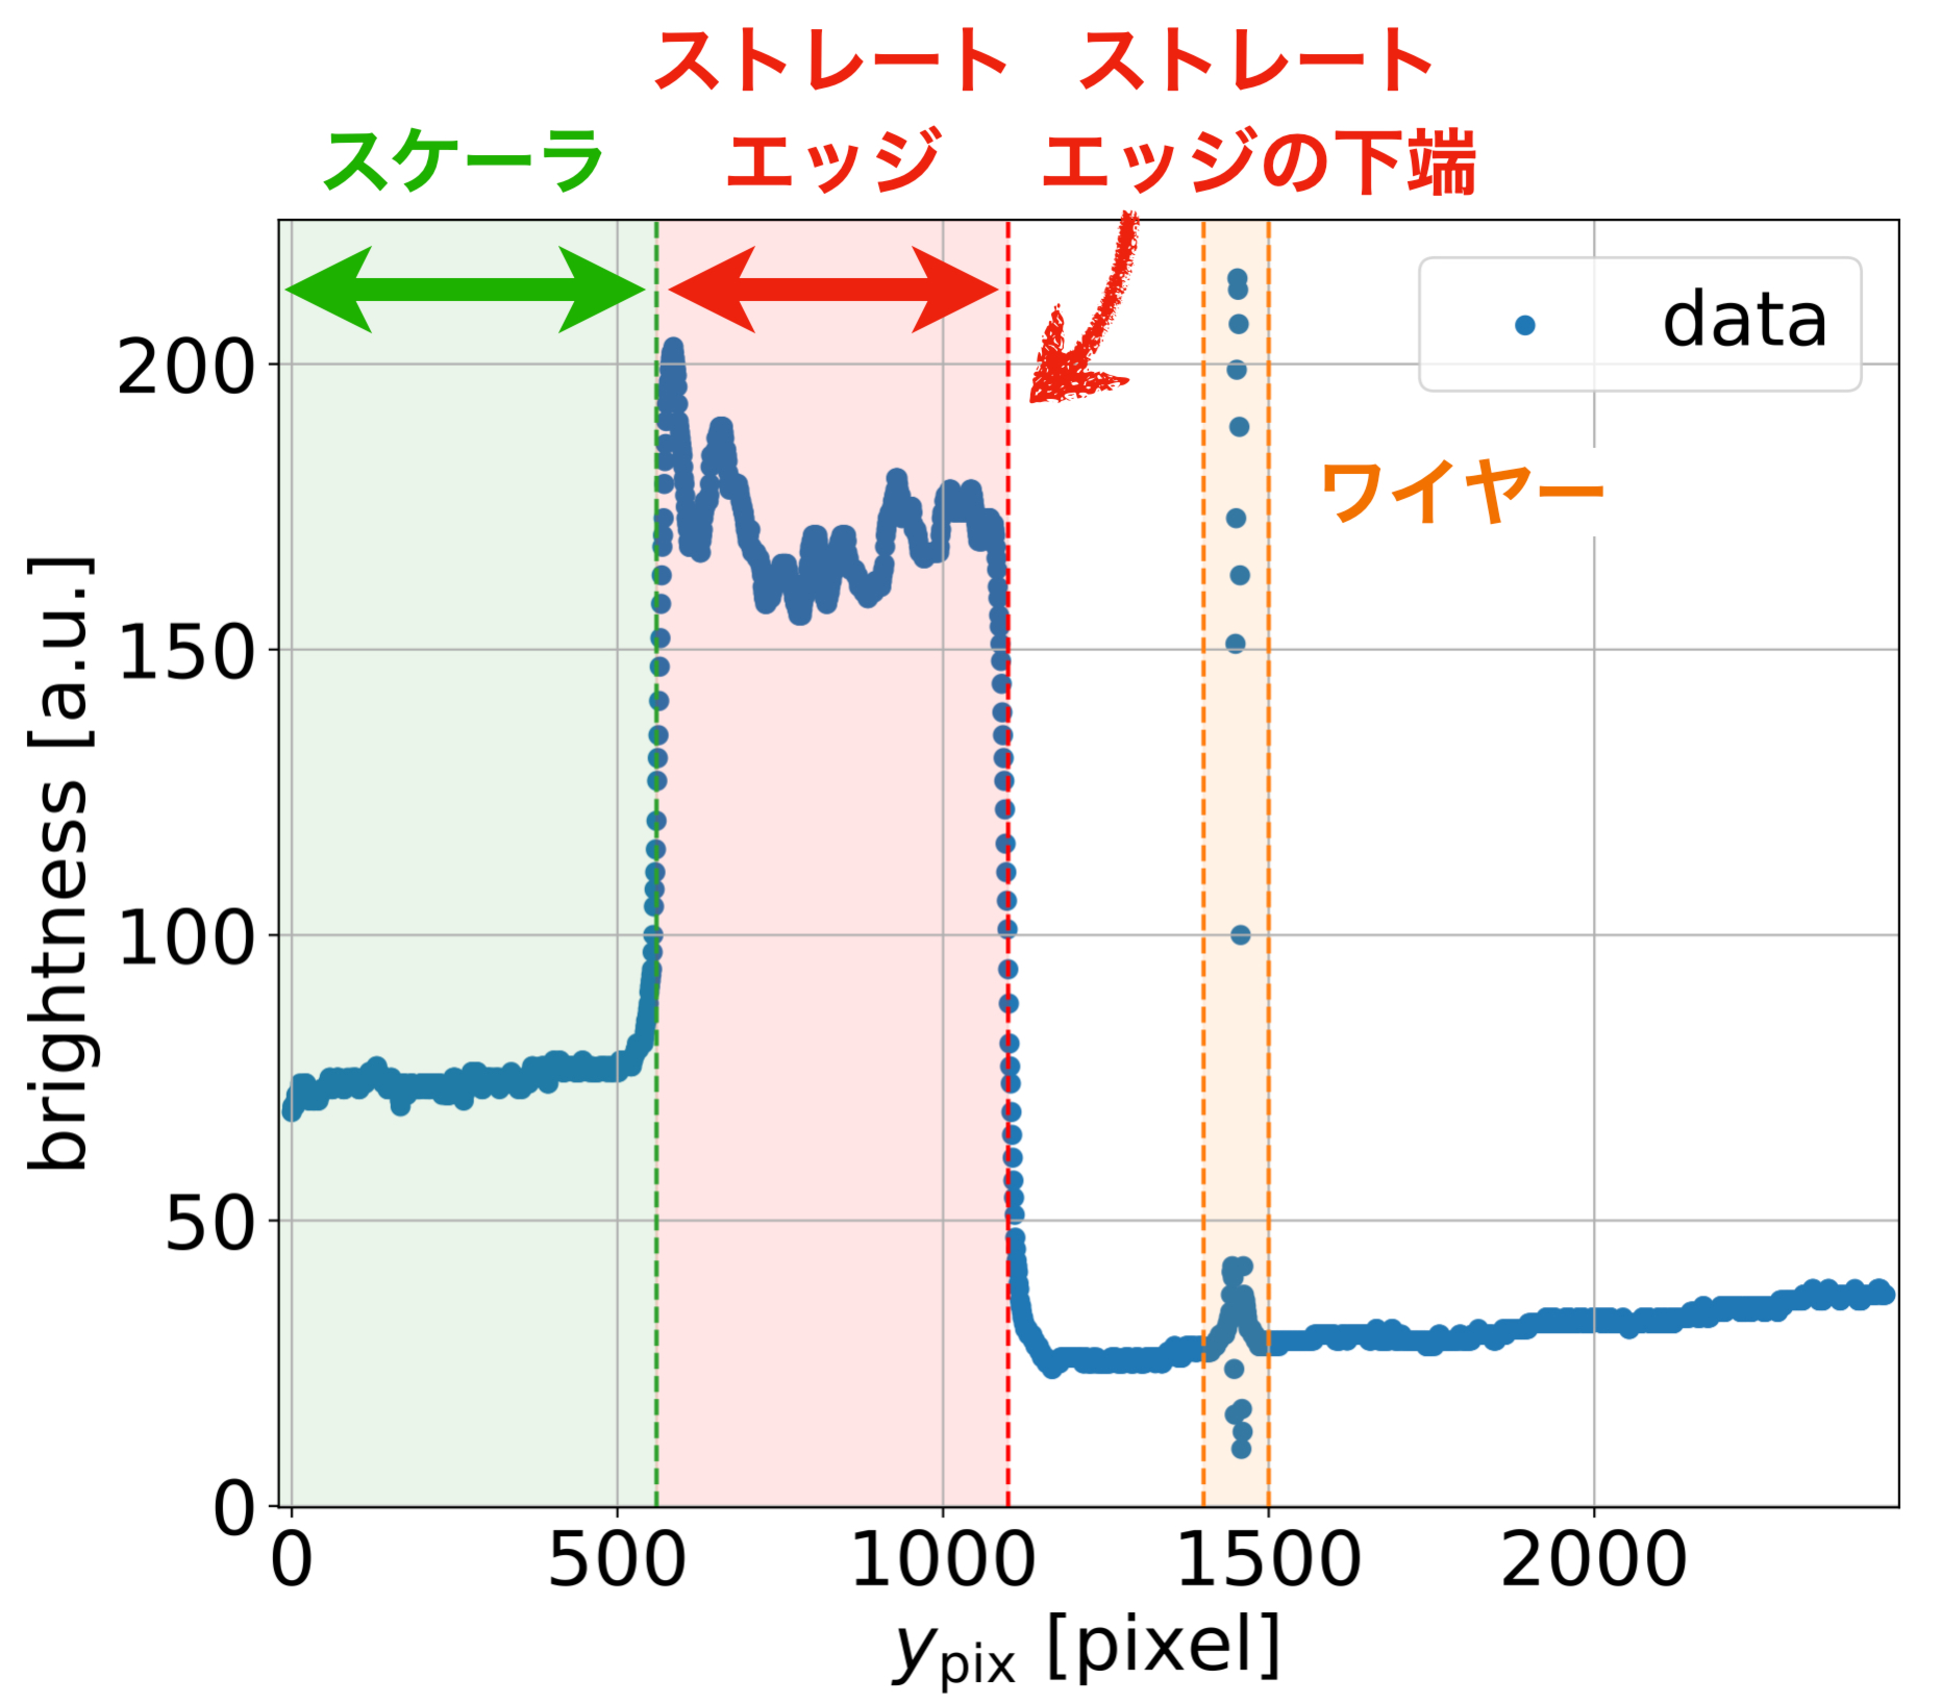
\includegraphics[width=0.8\textwidth]{wiresag/wiresag_edge_brightness.pdf}
    \caption{$x_{\mathrm{pix}}=\SI{1665}{pixel}$ における輝度の例}
    \label{fig:wiresag_edge_brightness}
\end{figure}
\subsubsection{ストレートエッジのfitting}
ストレートエッジの下端の輝度は、理想的な場合は階段関数的である。
実際にはカメラのピントによりぼやけてしまうため、シグモイド関数を用いてfittingを行う。
つまり、ストレートエッジの下端の輝度 $B_{\mathrm{SE}}(x)$ を
\begin{align}
    B_{\mathrm{SE}}(x;\,a,\,b,\,c,\,\text{offset}) = \dfrac{a}{1+\exp(-b(-x-c))} + \mathrm{offset}
\end{align}
としてfittingを行う。$a,\,b,\,c,\,\text{offset}$ は fitting parameter であり、$c$ はストレートエッジの下端の位置を表す。
図\ref{fig:wiresag_edge_fit}に実際にfittingした結果を示す。
\begin{figure}[H]
    \centering
    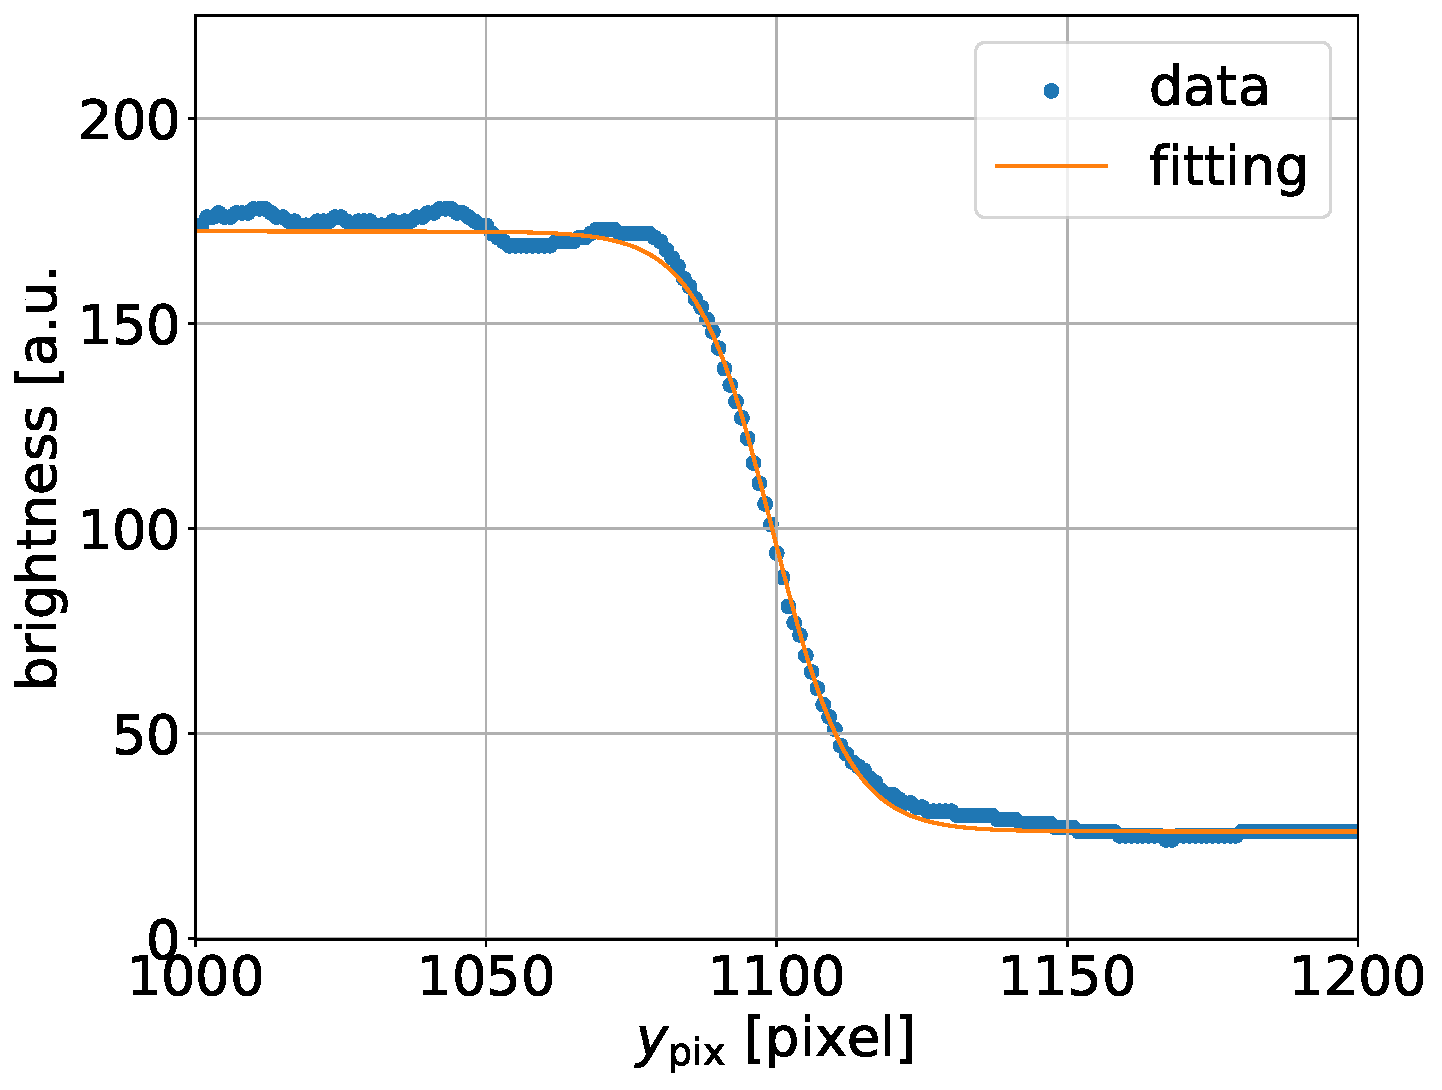
\includegraphics[width=0.8\textwidth]{wiresag/wiresag_straight_edge_fit.pdf}
    \caption{$x_{\mathrm{pix}}=\SI{1665}{pixel}$ におけるストレートエッジの輝度のfittingの結果の例}
    \label{fig:wiresag_edge_fit}
\end{figure}

\ref{subsec:wiresag_principle}にて述べた画像の回転を行うため、ストレートエッジの下端の fitting を $1132 < x_{\mathrm{pix}} < 2132$、
すなわち、中心から左右 $\SI{500}{pixel}$ の範囲に対して行い、ストレートエッジの位置を直線でfittingする。
図\ref{fig:wiresag_straight_edge}(\subref{fig:wiresag_straight_edge_positions_line})に、求めたストレートエッジの位置と、それを直線でfittingした結果を示す。
また、図\ref{fig:wiresag_straight_edge}(\subref{fig:wiresag_straight_edge_positions_rot})に、ストレートエッジの下端が水平になるように画像を回転させた結果を示す。
回転により、ストレートエッジが水平になっていることが確認できる。
回転後のストレートエッジの位置の標準偏差は、典型的に $\SI{1}{pixel}$ 程度であった。
\begin{figure}[H]
    \begin{minipage}[b]{0.5\hsize}
        \centering
        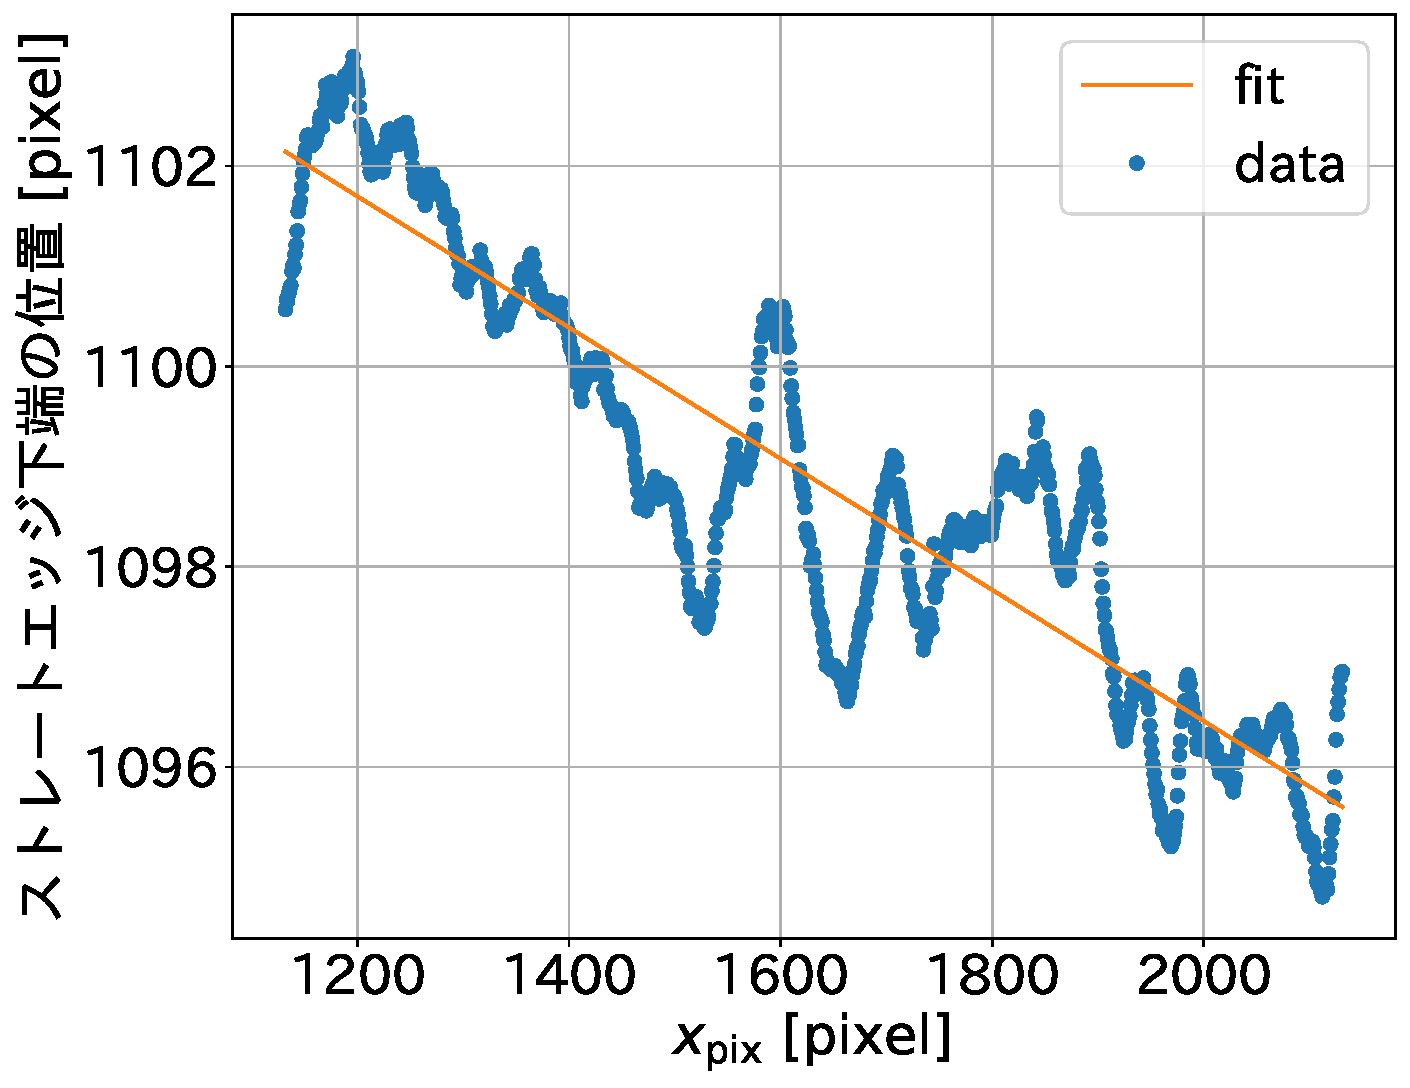
\includegraphics[width=0.97\textwidth]{wiresag/wiresag_straight_edge_positions_line.pdf}
        \subcaption{}
        \label{fig:wiresag_straight_edge_positions_line}
    \end{minipage}
    \begin{minipage}[b]{0.5\hsize}
        \centering
        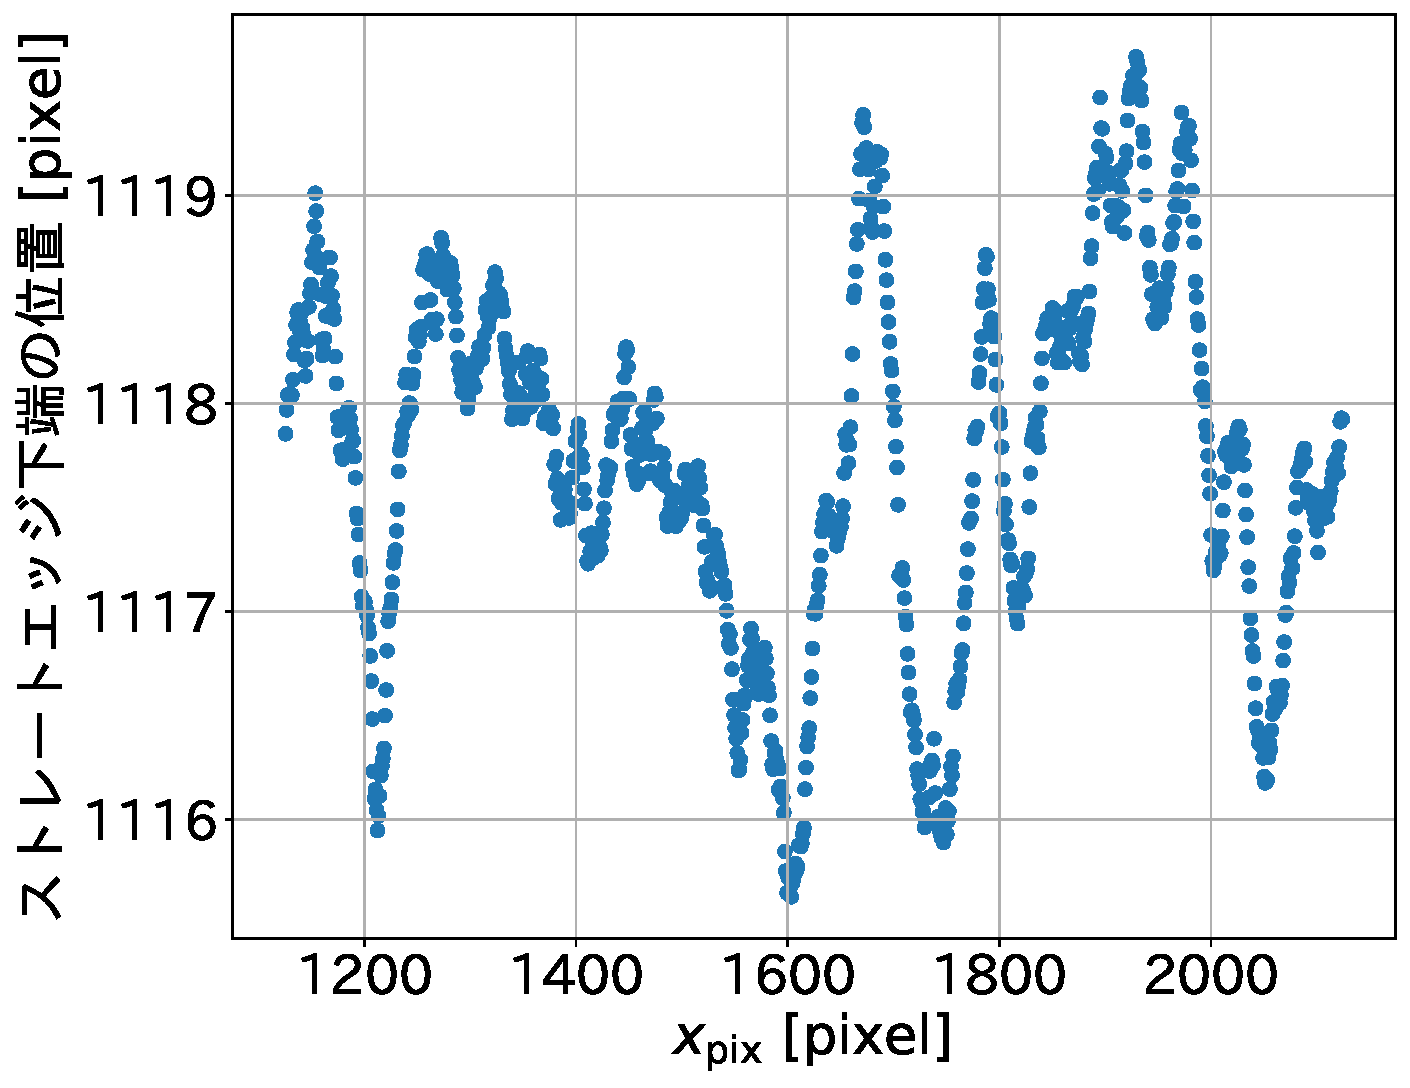
\includegraphics[width=0.97\textwidth]{wiresag/wiresag_straight_edge_positions_rot.pdf}
        \subcaption{}
        \label{fig:wiresag_straight_edge_positions_rot}
    \end{minipage}
    \caption{(\subref{fig:wiresag_straight_edge_positions_line}) 回転前のストレートエッジの位置と直線による fitting の結果の例
             (\subref{fig:wiresag_straight_edge_positions_rot}) 回転後のストレートエッジの位置の例
             }
    \label{fig:wiresag_straight_edge}
\end{figure}

\subsubsection{ワイヤーのfitting}
ワイヤーの輝度は理想的には階段関数的であり、急激に輝度を上げた後に急激に下げる。
しかし、ワイヤーの直径は $\SI{0.1}{mm}$ と短く、カメラのピントによりぼやけてしまうため、ガウス関数を用いて fitting を行う。
すなわち、ワイヤーの輝度 $B_{\mathrm{wire}}(x)$ を
\begin{align}
    B_{\mathrm{wire}}(x;\,A,\,\mu,\,\sigma,\,\text{offset}) = A\exp\qty(-\dfrac{(x-\mu)^2}{2\sigma^2}) + \mathrm{offset}
\end{align}
として fitting を行う。$A,\,\mu,\,\sigma,\,\text{offset}$ は fitting parameter であり、$\mu$ はワイヤーの中心の位置を表す。
図\ref{fig:wiresag_edge_target}におけるワイヤーの部分を実際にfittingした結果を図\ref{fig:wiresag_wire_fit}に示す。

一枚の画像に対して、$z$ は代表点として一つのみ算出するため、複数の $x_{\mathrm{pix}}$ に対してワイヤーの位置を求める必要がある。
たわみが大きいようなワイヤーに対しては、画像の中でもその位置を大きく変えてしまう。
これを考慮して、$1132 < x_{\mathrm{pix}} < 2132$ の範囲に対してワイヤーの位置を求める。
また、前項にて行ったストレートエッジを水平にするための回転をここでも行う必要がある。
回転前後のワイヤー位置を図\ref{fig:wiresag_wire_positions}に示す。
回転後のワイヤーの位置の標準偏差は、ワイヤーのたわみ方によって大きく異なるが、典型的には $\order{\SI{1}{pixel}}$ 程度であった。
\begin{figure}[H]
    \centering
    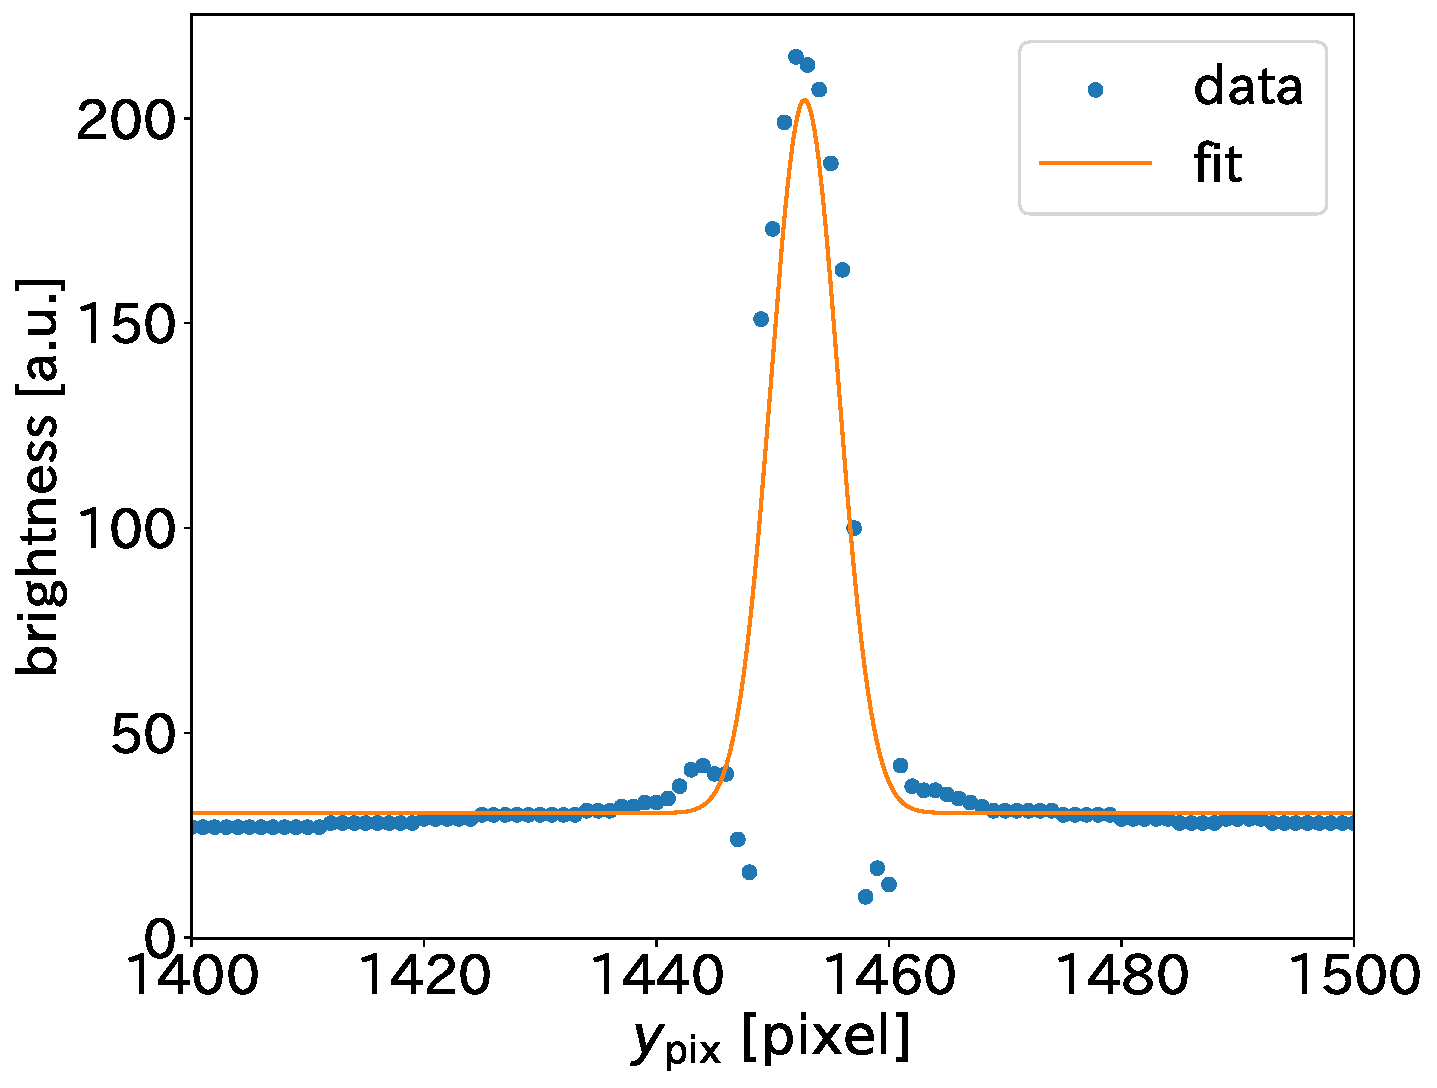
\includegraphics[width=0.8\textwidth]{wiresag/wiresag_wire_fit.pdf}
    \caption{$x_{\mathrm{pix}}=\SI{1665}{pixel}$ におけるワイヤーの輝度のfittingの結果の例}
    \label{fig:wiresag_wire_fit}
\end{figure}
\begin{figure}[H]
    \begin{minipage}[b]{0.5\hsize}
        \centering
        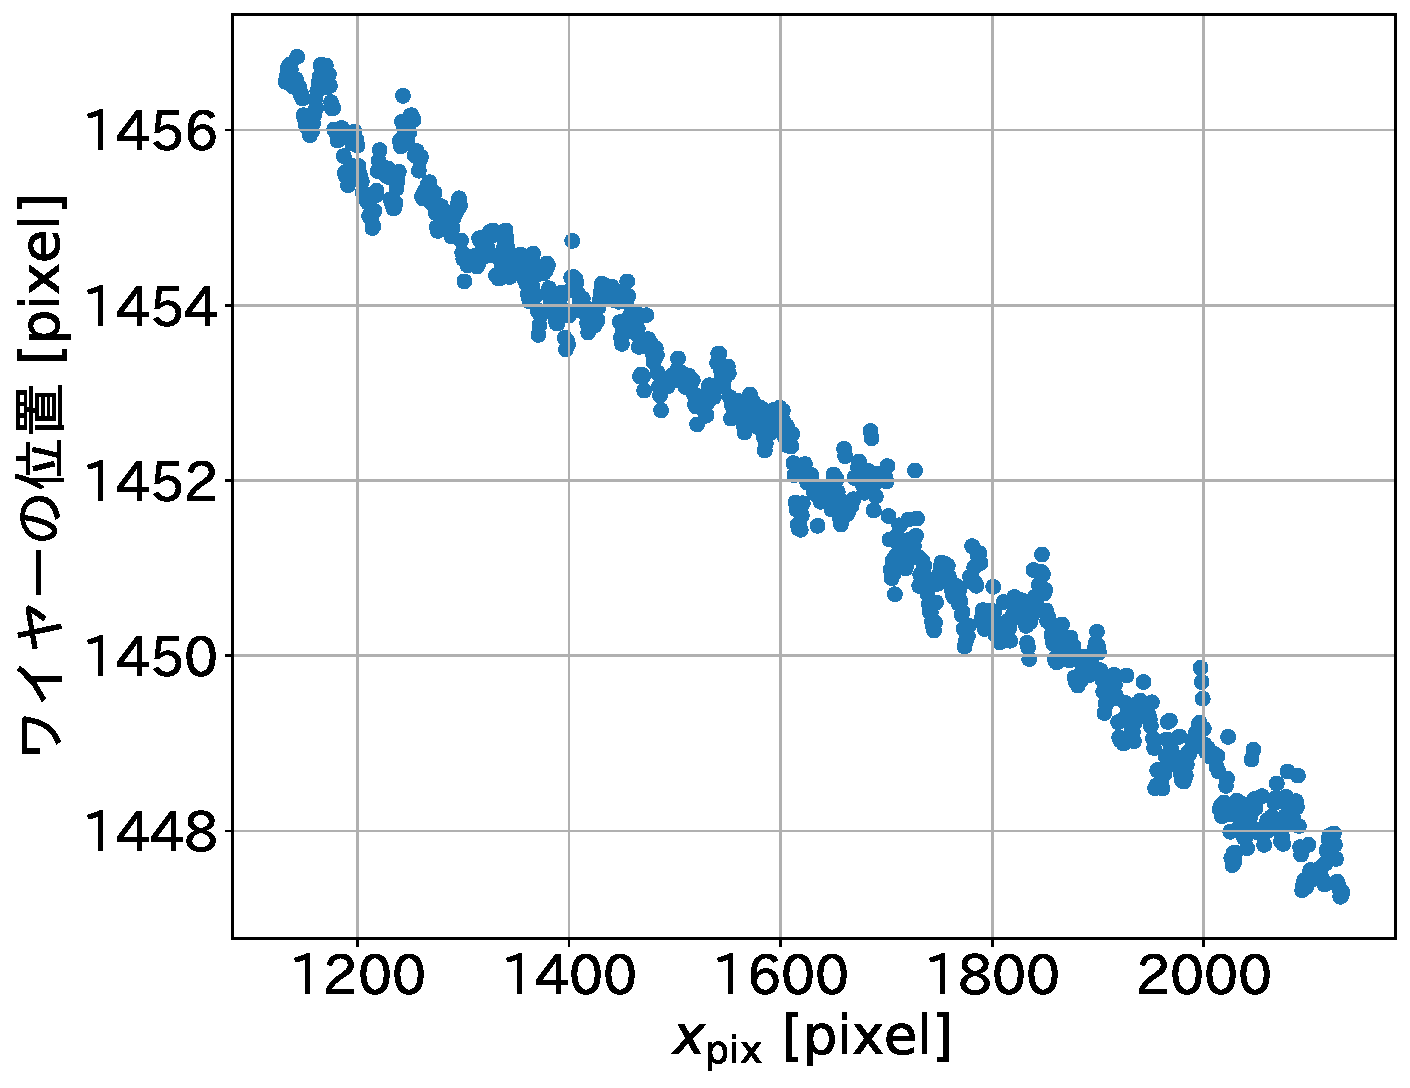
\includegraphics[width=0.97\textwidth]{wiresag/wiresag_wire_positions.pdf}
        \subcaption{}
        \label{fig:wiresag_wire_positions_line}
    \end{minipage}
    \begin{minipage}[b]{0.5\hsize}
        \centering
        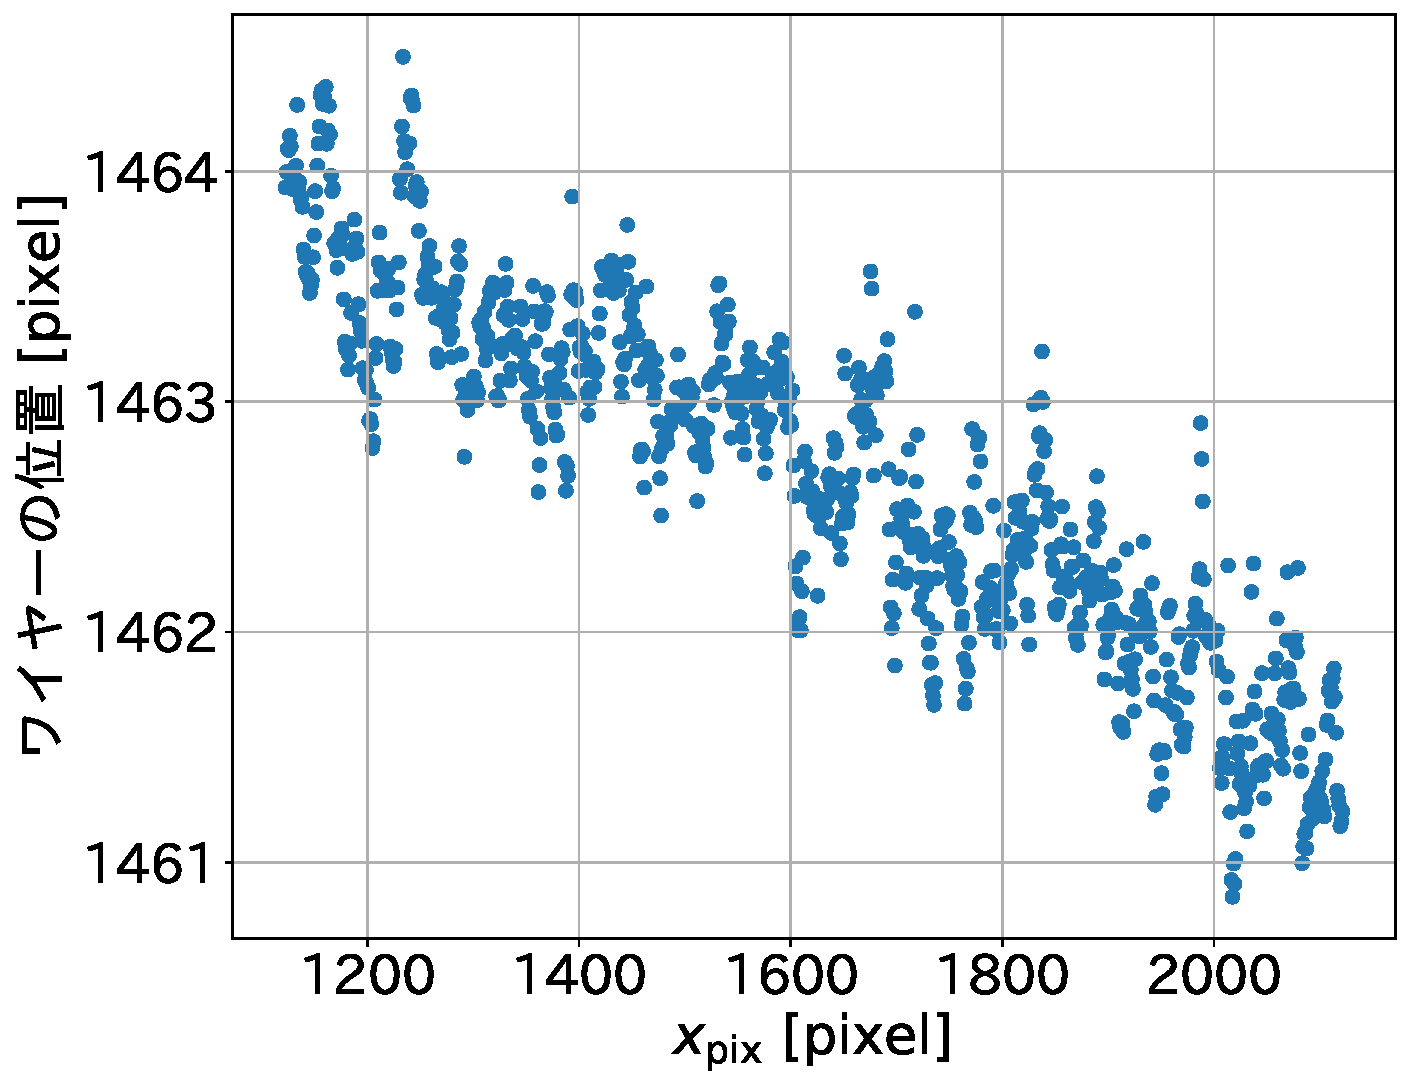
\includegraphics[width=0.97\textwidth]{wiresag/wiresag_wire_positions_rot.pdf}
        \subcaption{}
        \label{fig:wiresag_wire_positions_rot}
    \end{minipage}
    \caption{(\subref{fig:wiresag_wire_positions_line}) 回転前のワイヤーの位置の例
             (\subref{fig:wiresag_wire_positions_rot}) 回転後のワイヤーの位置の例
             }
    \label{fig:wiresag_wire_positions}
\end{figure}

\subsection{$z$ の算出}
前々項にて求めた回転後のストレートエッジの位置と、前項にて求めたワイヤーの位置から $z$ を算出する。
図\ref{fig:wiresag_wire_se_positions_diff}に、回転後のワイヤーの位置からストレートエッジの位置を引いた値 $y_{\mathrm{wire}}-y_{\mathrm{SE}}$ を示す。
この平均を取ることで、代表的な $z$ と誤差(標準偏差) $\delta z$ を得る。
今回の例の場合、
\begin{align}
    z &= \SI{500}{pixel} \\
    \delta z &= \SI{1}{pixel}
\end{align}
であった。
スケーラのfittingによれば、1 pixel が対応する長さおよそ $\SI{5.78}{\mu m}$ であった。
これを用いて $z$ と $\delta z$ を実際の長さに変換すると
\begin{align}
    z &= \SI{2890}{\mu m} \\
    \delta z &= \SI{6}{\mu m}
\end{align}
となる。ここで得られた $\delta z$ は、統計的な誤差によるものである。
このようにして、撮影された画像から代表点として$z$を一つ算出することができる。
\begin{figure}[H]
    \centering
    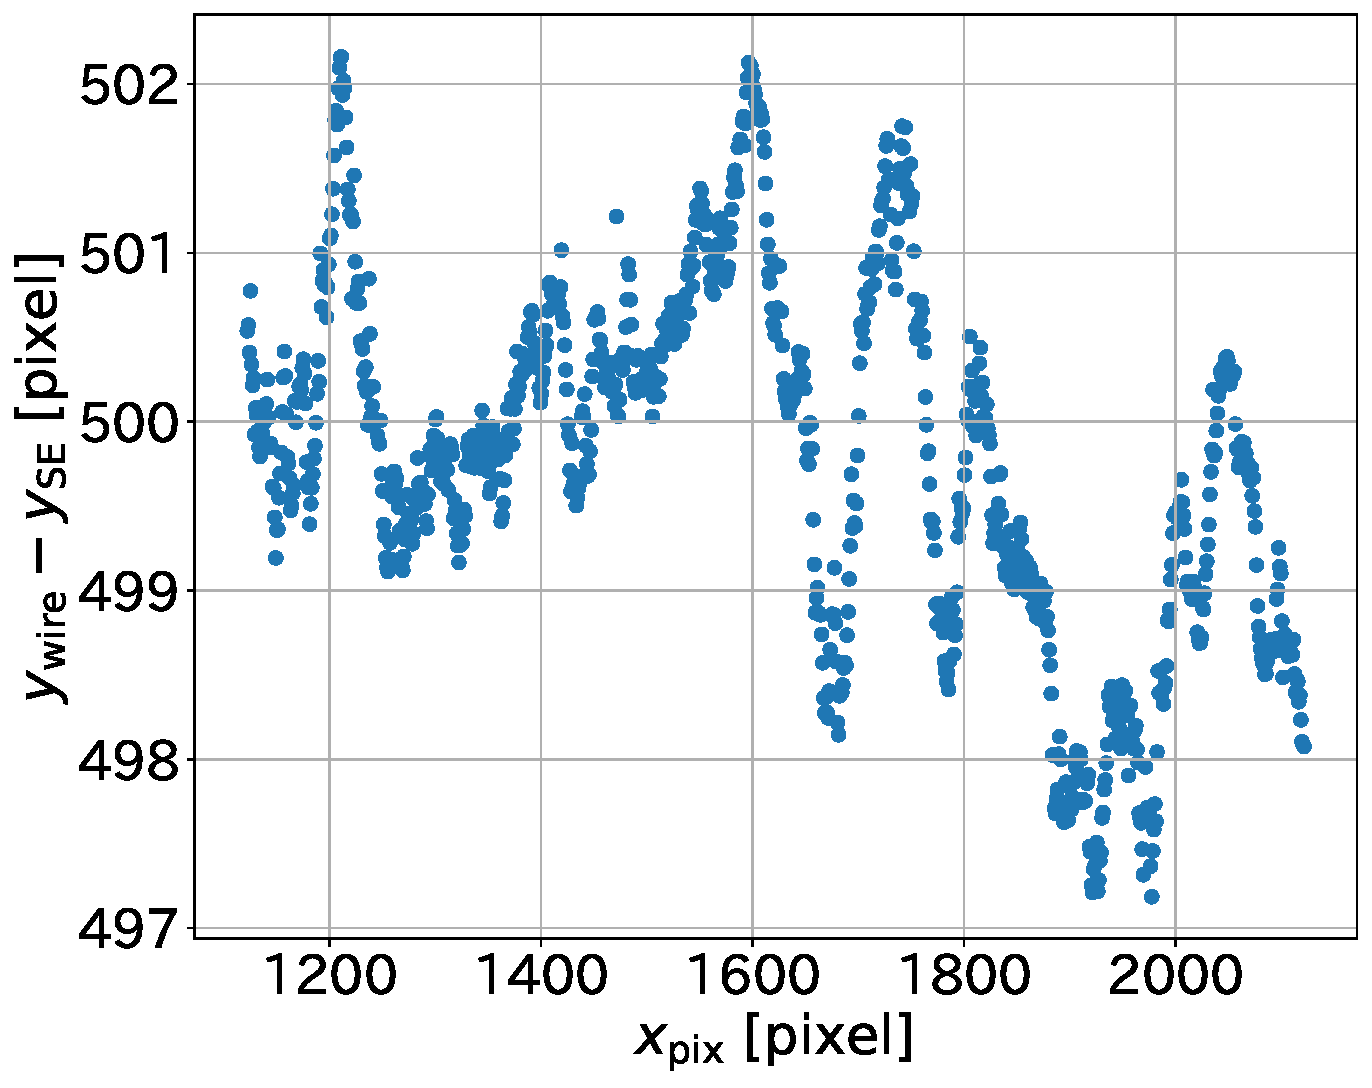
\includegraphics[width=0.7\textwidth]{wiresag/wiresag_wire_se_positions_diff.pdf}
    \caption{回転後のワイヤーの位置からストレートエッジの位置を引いた値の例}
    \label{fig:wiresag_wire_se_positions_diff}    
\end{figure}
\subsection{カテナリーでのfitting}
一本のワイヤーに対して複数の写真を撮り、それぞれの写真から得られた$z$をカテナリー曲線でfittingすることで、ワイヤーのたわみ量を算出する。
このとき、fittingに用いるカテナリーは式\eqref{eq:wiresag_catenary_tilt}で表されるものである。
ただし、式\eqref{eq:wiresag_catenary_tilt}ではワイヤーの左端が $(0,\,0)$ に位置していることを仮定していたので、
これを並行移動する自由度を入れることで、より一般的なカテナリー曲線を得る。
すなわち、fittingに用いるカテナリー曲線は
\begin{align}
    f_{\mathrm{tilt}}(x;a,\,X,\,Y,\,x_{\mathrm{offset}},\,y_{\mathrm{offset}}) &= a\cosh\qty(\dfrac{x+x_{\mathrm{offset}}+c_1}{a}) + c_2 - y_{\mathrm{offset}}\\
    c_1 &= a\sinh^{-1}\qty[\dfrac{Y}{2a\sinh\qty(\dfrac{X}{2a})}] \\
    c_2 &= -a\cosh\qty(\dfrac{c_1}{a})
\end{align}
となる。fitting parameterは$a,\,X,\,Y,\,x_{\mathrm{offset}},\,y_{\mathrm{offset}}$であり、
$X,\,Y$ の間には、式\eqref{eq:wiresag_frame_length}によりワイヤーに対して定まる$L_{\mathrm{frame}}$を用いて
\begin{align}
    L_{\mathrm{frame}} &= \sqrt{X^2+Y^2}
\end{align}
という拘束条件がある。また、$z$ は距離を表しているので
\begin{align}
    z_{i} &= -f_{\mathrm{tilt}}(x_{i};\,a,\,X,\,Y,\,x_{\mathrm{offset}},\,y_{\mathrm{offset}})
\end{align}
としてfittingを行う。
図\ref{fig:wiresag_catenary}に、$z$ とカテナリー曲線でfittingした結果を示す。
$z$ の誤差としては、評価系の設計から生まれる誤差 $\SI{49}{\mu m}$ と、fittingここまでの処理で得られた誤差を考えた。
このfittingにより求めた $a$ を式\eqref{eq:wiresag_sag}に代入することで、ワイヤーのたわみ量 $d_{\mathrm{sag}}$ を得る。
さらに、求めた $d_{\mathrm{sag}}$ を式\eqref{eq:wiresag_sag_angle}に代入することで、ワイヤーのたわみ角を得る。
今回の例では
\begin{align}
    d_{\mathrm{sag}} &= 275 \pm \SI{5}{\mu m} \\
    \theta_{\mathrm{sag}} &= 0.041\tcdegree \pm 0.0007 \tcdegree
\end{align}
を得た。
\begin{figure}[H]
    \centering
    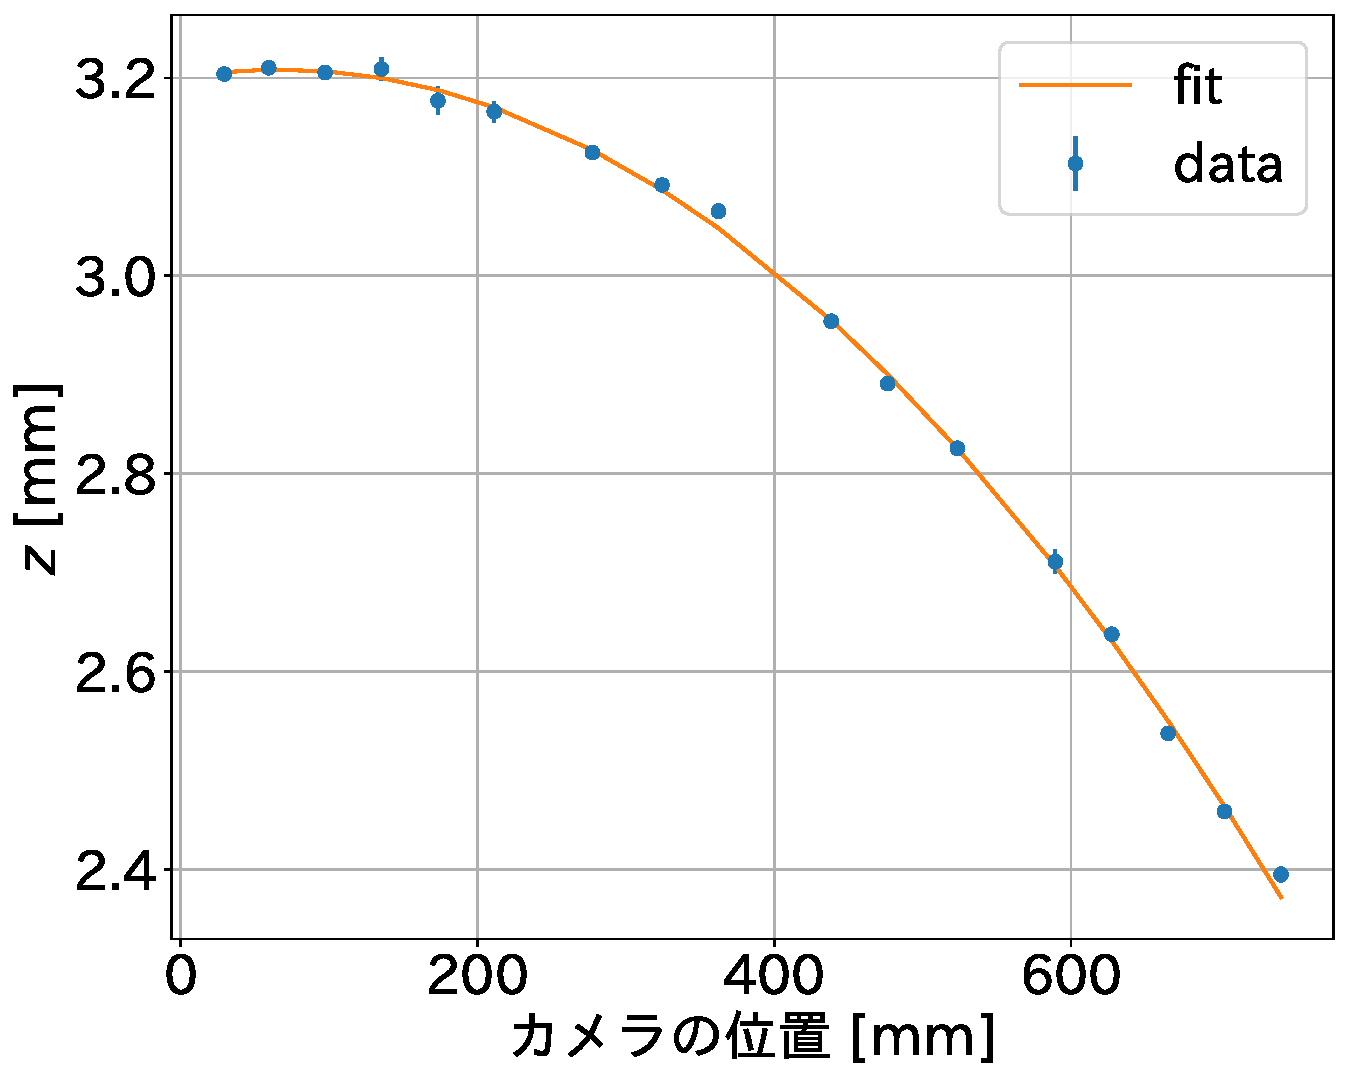
\includegraphics[width=0.75\textwidth]{wiresag/wiresag_catenary.pdf}
    \caption{カテナリー曲線で fitting した結果の例}
    \label{fig:wiresag_catenary}
\end{figure}
\section{開発した評価系の性能評価}
\subsection{評価手法}
これまで述べてきた手法の性能評価として、張力を変えながらのたわみ量を測定する。
評価系に図\ref{fig:wiresag_performance_zig}のような治具をつけ、治具の溝に沿うようにワイヤーを張る。
溝は水平方向と鉛直方向を滑らかに接続しており、鉛直方向に出てきたワイヤーにフックをつけ、
フックに重りをつけることでワイヤーの張力を調節できるようになっている。
実際に評価系に治具を取り付け、ワイヤーを張ったときの様子を図\ref{fig:wiresag_performance_cehck_system}に示す。
このとき、張られたワイヤーの両端間の距離は$\SI{757}{mm}$で、
重りは$\SI{57}{g},\,\SI{69}{g},\,\SI{85}{g},\,\SI{102}{g},\,\SI{122}{g},\,\SI{158}{g},\,\SI{178}{g},\,\SI{190}{g},\,\SI{218}{g},\,\SI{228}{g},\,\SI{239}{g},\,\SI{250}{g}$のものを使用した。
\begin{figure}[H]
    \centering
    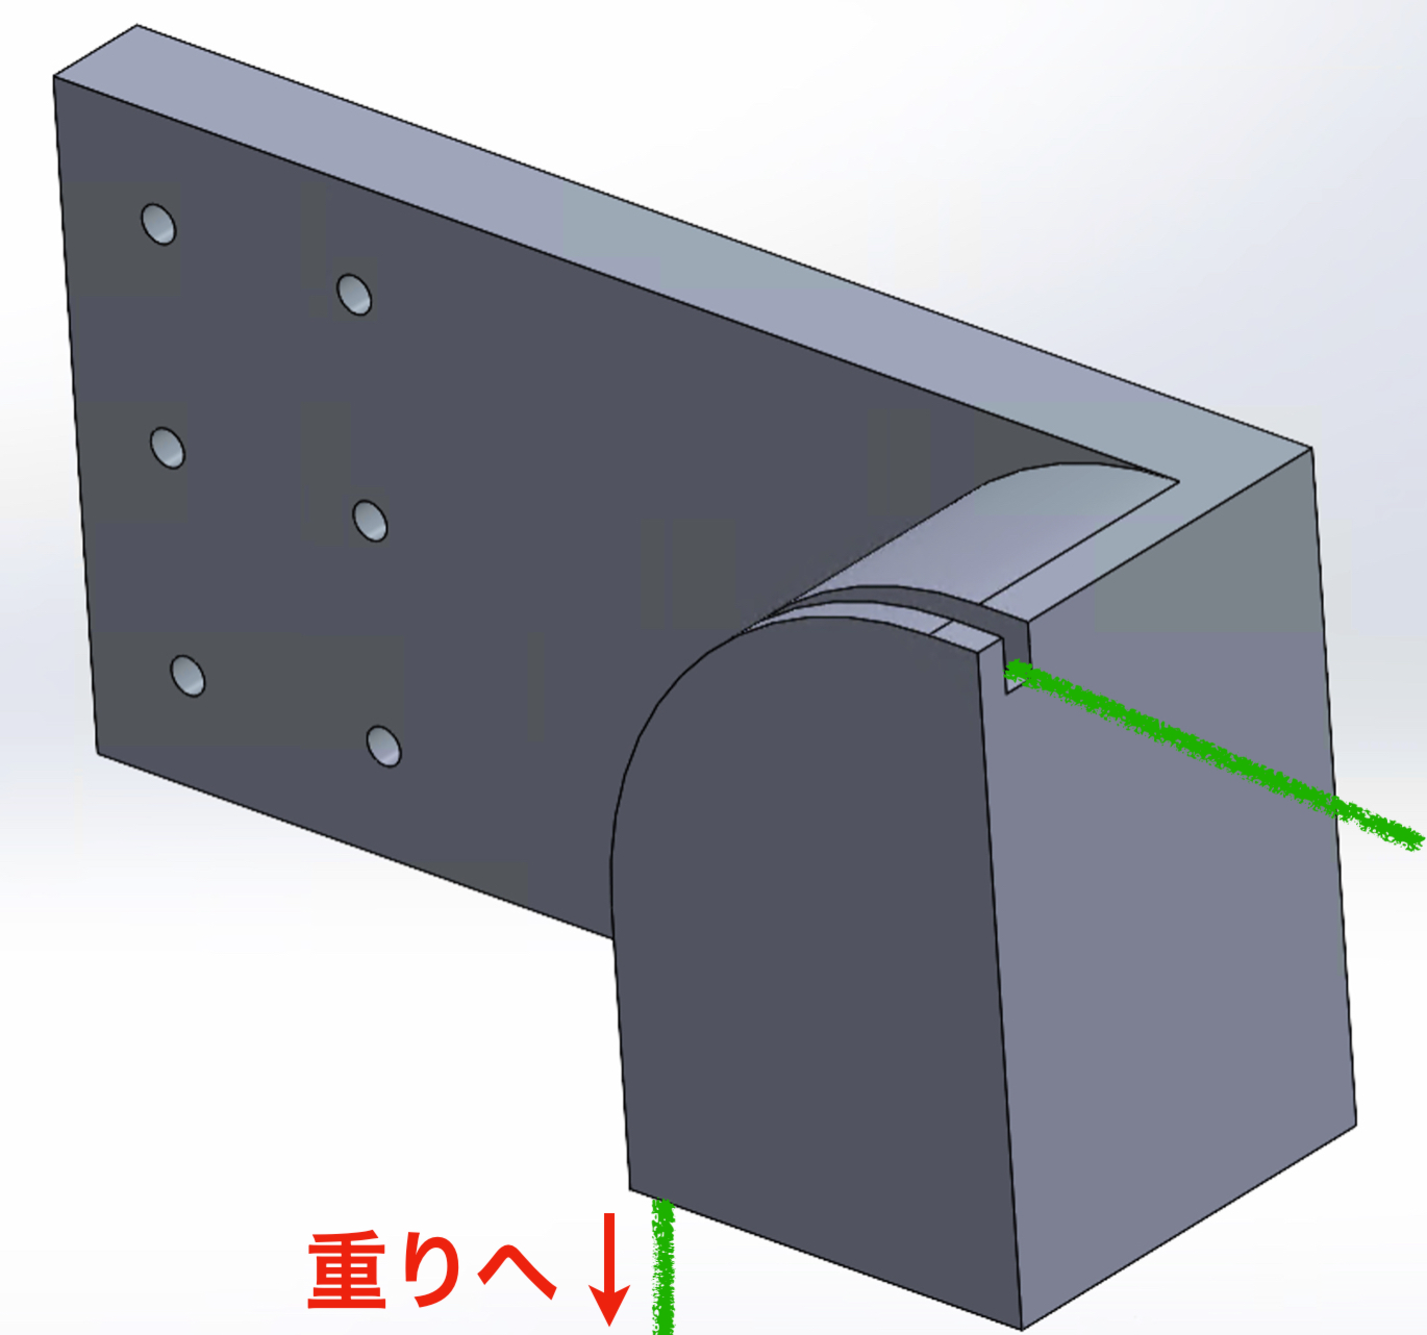
\includegraphics[width=0.6\textwidth]{wiresag/wiresag_performance_zig.pdf}
    \caption{張力を変えた時のたわみの変化の原理検証の概念図}
    \label{fig:wiresag_performance_zig}
\end{figure}
\begin{figure}[H]
    \centering
    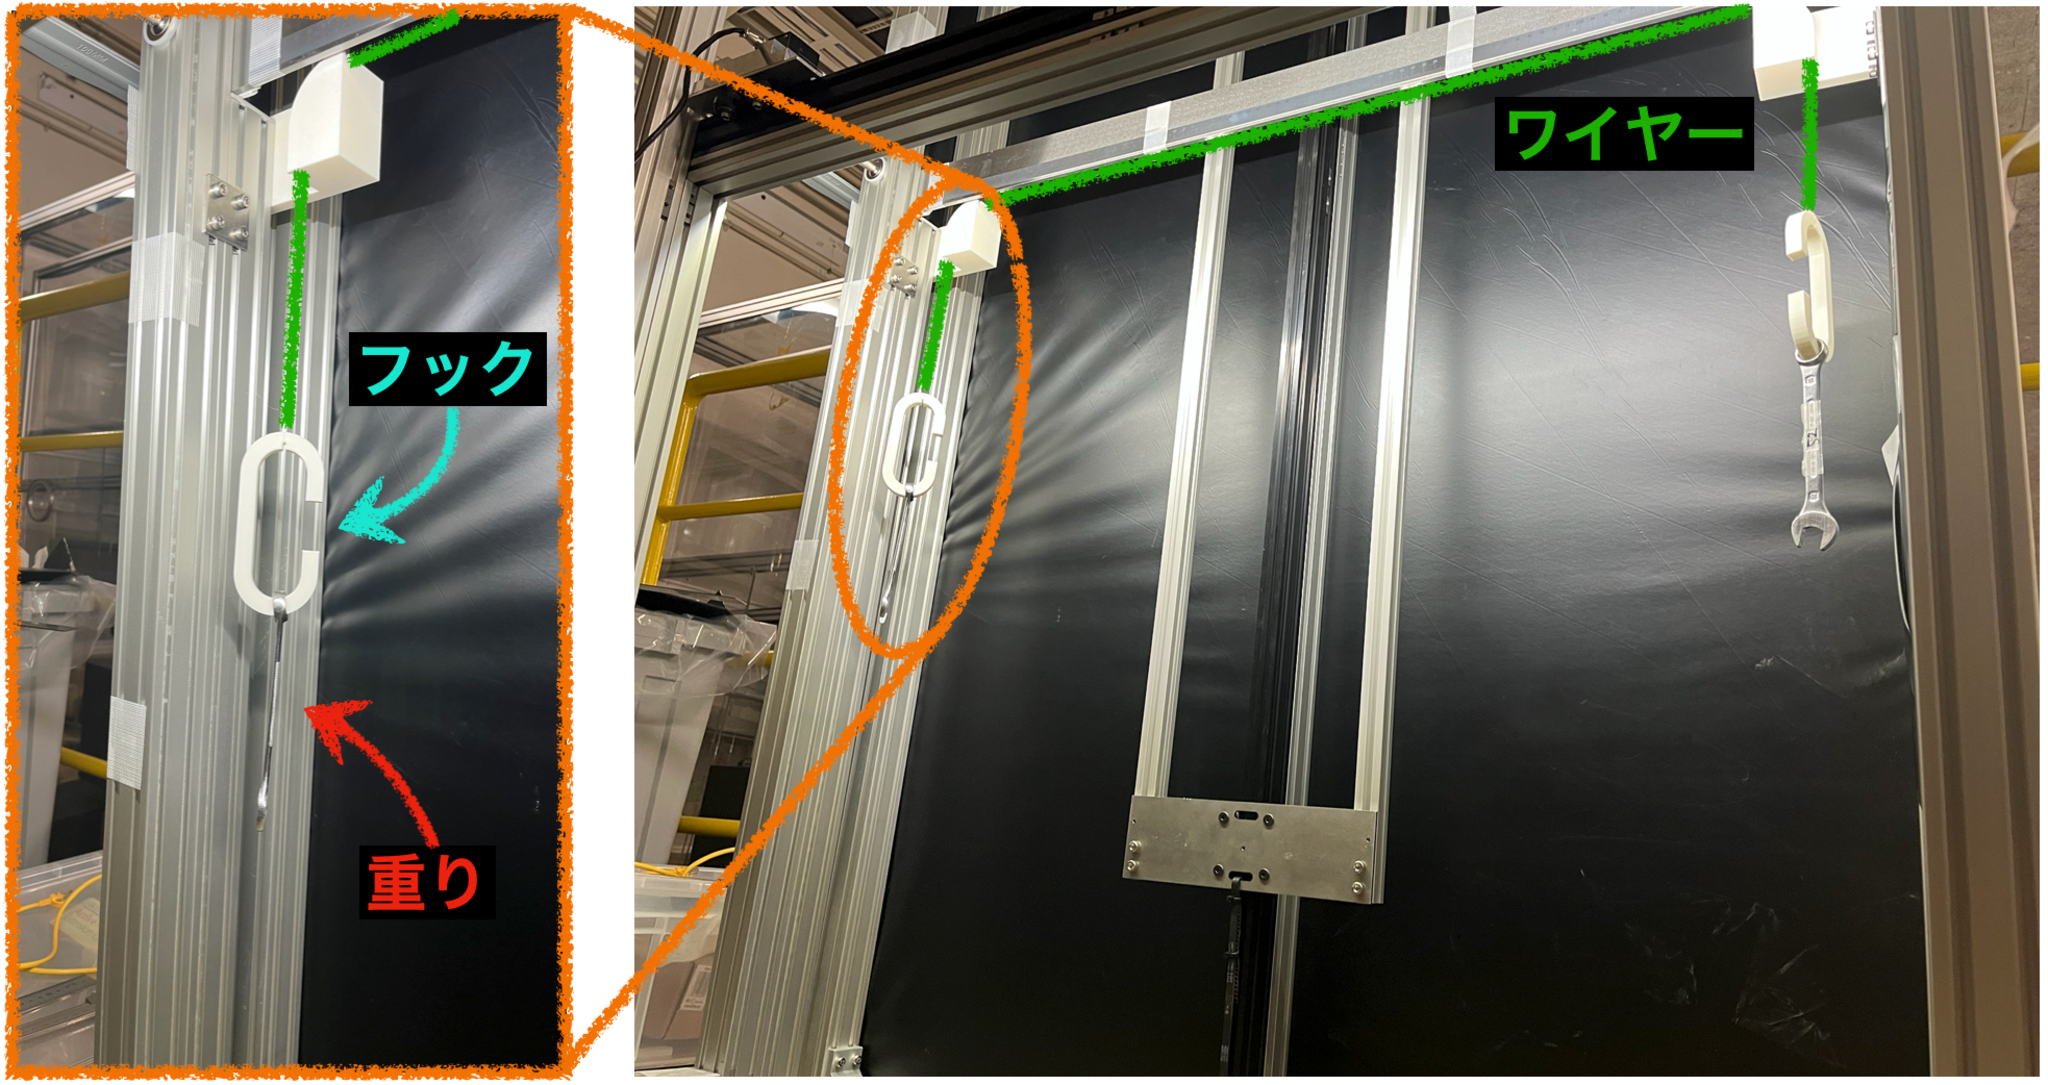
\includegraphics[width=0.95\textwidth]{wiresag/wiresag_performance_check_system.pdf}
    \caption{作成した評価系の原理検証のための測定時の様子}
    \label{fig:wiresag_performance_cehck_system}    
\end{figure}

\subsection{評価結果とその考察}
図\ref{fig:wiresag_performance_check_result}に張力を変えた時の評価されたたわみ量の遷移を示す。
横軸は吊るした重りの重さ、縦軸はワイヤーのたわみ量を示している。
青点は評価されたたわみ量を表し、オレンジの線はワイヤーの長さと重りの重さを決めることで
式\eqref{eq:wiresag_sag_angle}より求められる理論的なたわみ量を表している。
また、参考としてスパースワイヤーグリッドのワイヤーを張る時に使う重りの重さ$\SI{230}{g}$のところに点線を入れている。
この結果から、得られた評価値と理論値の差は最大で$\SI{50}{\mu m}$程度であるとわかった。
そのため、この評価系で評価されるたわみ量の精度は、$\SI{50}{\mu m}$程度であると結論づける。
\begin{figure}[H]
    \centering
    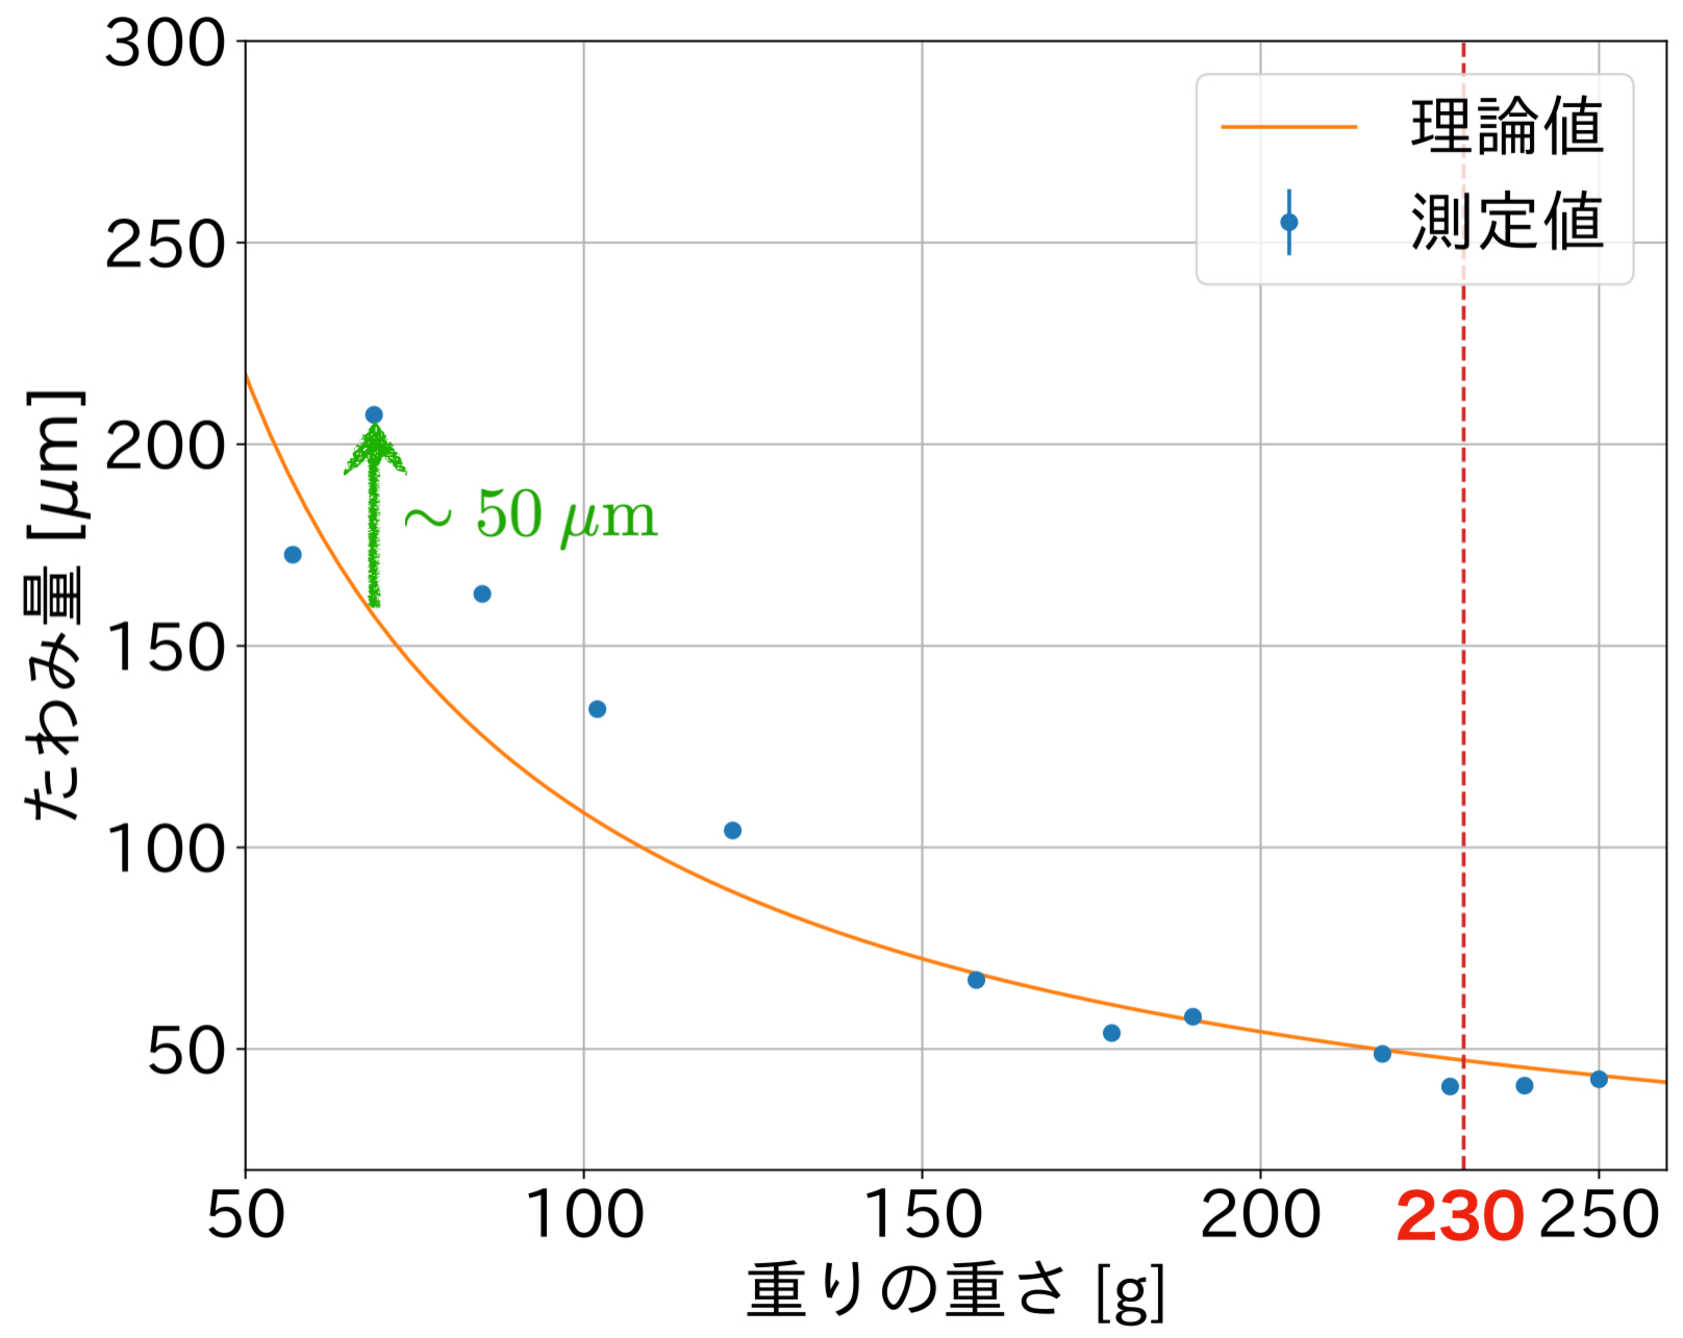
\includegraphics[width=0.8\textwidth]{wiresag/wiresag_performance_check_result.pdf}
    \caption{張力を変えた時のたわみ量の変化}
    \label{fig:wiresag_performance_check_result}
\end{figure}
\subsection{得られた誤差の考察}
\subsection{評価系の光学系を考慮した $z$ の測定原理}
図\ref{fig:wiresag_concept_yoko}にワイヤーのたわみ量の評価原理の横から見た概念図を示す。
これは過去の手法における概念図\ref{fig:wiresag_setup_old}を新しい系に合わせて変更したものであり、
カメラから見るとストレートエッジが手前に位置し、ワイヤーがその奥に位置するような配置になっている。
各パラメータの意味とその値、誤差を表\ref{tab:wiresag_concept_yoko_params}に示す。
この系において、測定される量 $z'$ を用いてストレートエッジとワイヤー間の距離 $z$ を表すと、
\begin{align}
    z = \dfrac{z'}{\cos\phi} + \alpha\tan\phi \\
    \phi = \arctan\qty(\dfrac{L_{\mathrm{camera}}}{\alpha})
\end{align}
となるが、今、$L_{\mathrm{camera}}$は$\SI{0}{mm}$であるため、
\begin{align}
    z = z'
\end{align}
として問題ない。

\begin{figure}[H]
    \centering
    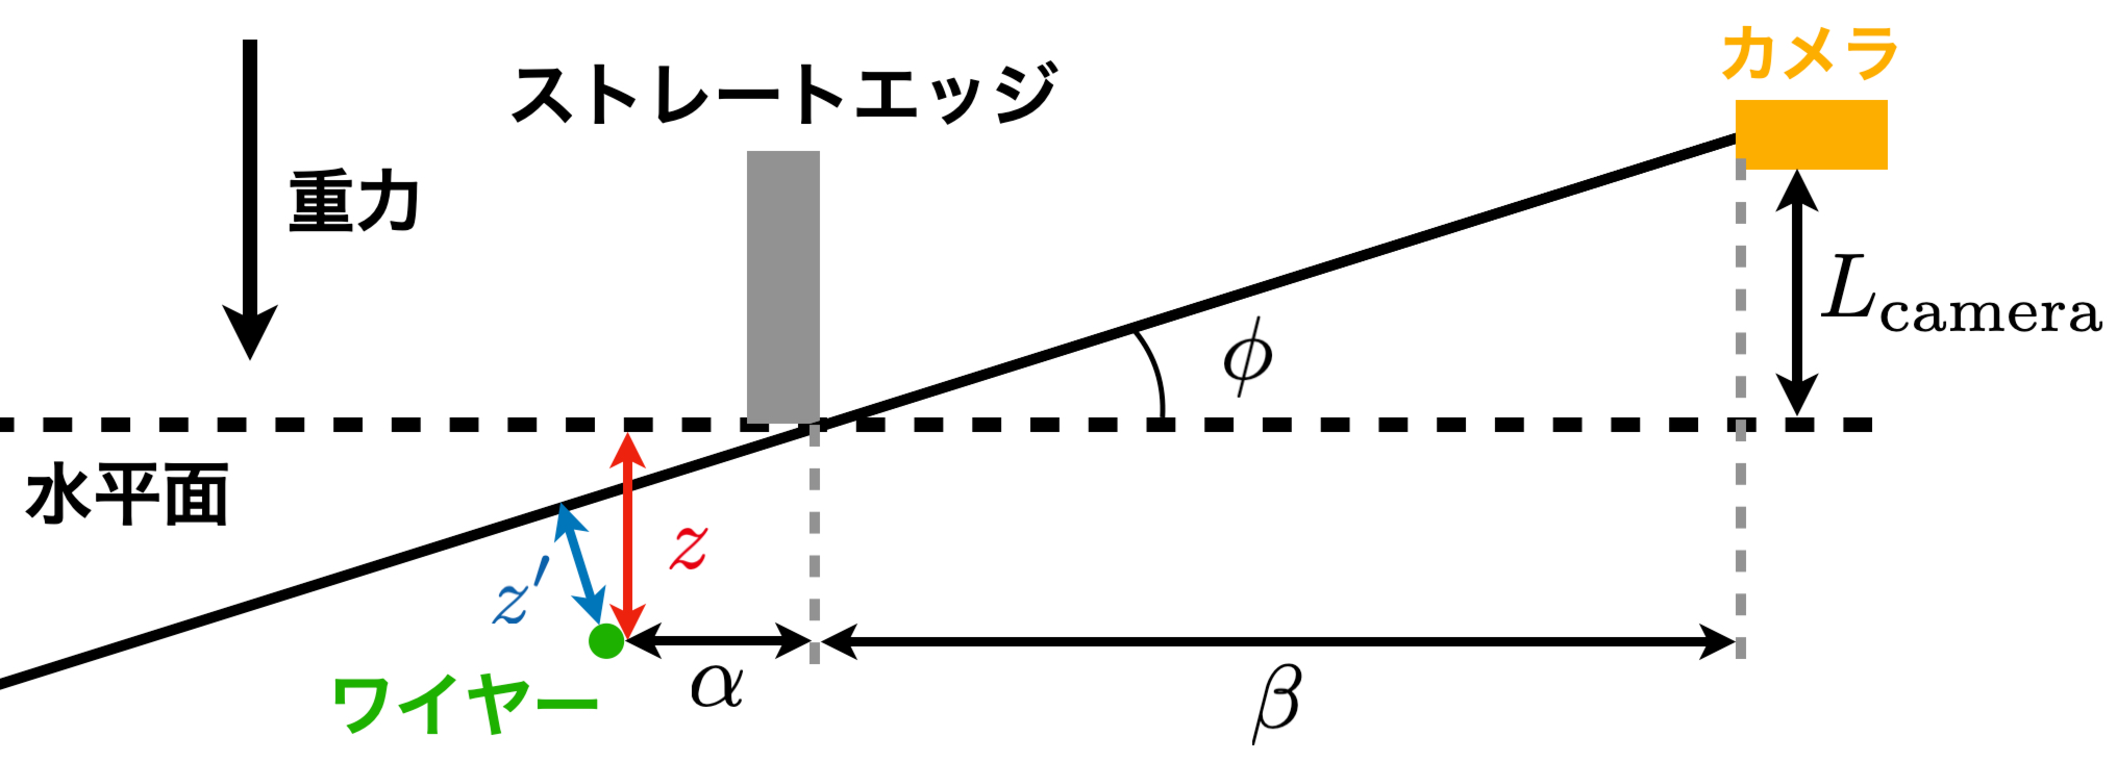
\includegraphics[width=0.8\textwidth]{wiresag/wiresag_concept_yoko.pdf}
    \caption{ワイヤーのたわみ量の評価原理の横から見た概念図}
    \label{fig:wiresag_concept_yoko}
\end{figure}
\begin{table}[H]
    \centering
    \caption{図\ref{fig:wiresag_concept_yoko}における各パラメータの意味と値}
    \begin{tabular}{cccc}
        \hline
        パラメータ & 意味 & 値 & 誤差 \\
        \hline\hline
        $\alpha$ & ストレートエッジとワイヤーまでの水平距離 & $\SI{15}{mm}$ & $\pm\SI{2}{mm}$ \\
        $\beta$ & ストレートエッジからカメラまでの水平距離 & $\SI{205}{\mm}$ & $\pm\SI{5}{mm}$ \\
        $L_{\mathrm{camera}}$ & ストレートエッジ下端の面からカメラまでの鉛直距離 & $\SI{0}{mm}$ & $\pm\SI{0.5}{mm}$ \\
        \hline
    \end{tabular}
    \label{tab:wiresag_concept_yoko_params}
\end{table}

\subsection{評価系の設計から生まれる $z$ の誤差の見積もり}
過去の手法においては、$\phi$ が典型的に $5\tcdegree$ 程度と小さくない値であったために、
$L_{\mathrm{camera}}$ や $\alpha$ から $z$ へ大きな誤差が生じていた\cite{swg:murata}。
この誤差を抑えるためには、$\phi$ を小さくすることが重要であるが、
過去の評価系ではスパースワイヤーグリッドを水平面上に設置して撮影しており、
他のワイヤーが撮影対象のワイヤーに重なってしまうため $\phi\sim 0\tcdegree$、すなわち 
$L_{\mathrm{camera}} \sim \SI{0}{mm}$ で撮影することができなかった(図\ref{fig:wiresag_picture_old})。
これを解決するため、スパースワイヤーグリッドを鉛直方向に立てて撮影を行うことで、$L_{\mathrm{camera}}=0\pm\SI{0.5}{mm}$ で撮影を行い、誤差の低減を図った。
新しい評価系において、$z$ の誤差は
\begin{align}
    \delta z = \sqrt{\qty(\dfrac{1}{\cos\phi})^2\delta z'^2 + \qty(\dfrac{\tan\phi}{\cos\phi}+\dfrac{\alpha}{\cos^2\phi})^2\delta\phi^2 + \tan^2\phi\delta\alpha^2}
\end{align}
と表され、表\ref{tab:wiresag_concept_yoko_params}に示したパラメータの誤差を代入すると、
\begin{equation}
    \delta z \sim \SI{39}{\mu m}
\end{equation}
となる。$z'$ の誤差についてはカメラの $\SI{1}{pixel}$ が対応する長さであり、
次節の解析にて明らかになるがこれは典型的に $5\sim\SI{6}{\mu m}$ 程度である。
また、$z$ にはストレートエッジの真直度由来の誤差 $\SI{30}{\mu m}$ が含まれるため、これも考慮に入れると $z$ の誤差は
\begin{equation}
    \delta z = \sqrt{39^2+30^2}\ \mu\mathrm{m} = \SI{49}{\mu m}
\end{equation}
程度だと見積もられる。
\section{スパースワイヤーグリッドのたわみ量の評価}
\subsection{評価手法}
作成した評価系を用いて、スパースワイヤーグリッドのたわみ量を評価する。
スパースワイヤーグリッドには\ref{}項で述べたように$\SI{230}{g}$の重りを使用し、
ワイヤー番号が奇数番目のものと偶数番目のものに分け、二回に分けてワイヤーを張ることで作成された。

\end{document}